\section{Outline of the Appendix}
%
In the appendix, we list the posteriors and remaining sampling steps for of the $\MCMC$ sampling algorithm for the $\QVP$ and $\NCQVP$ models discussed in the paper in Section~\ref{app:qvp-posteriors}. We additionally give sampling steps for a MCMC-sampler in Section~\ref{app:asis} which interweaves the posterior sampling steps for the centred and non-centred parameterisation in the sense of \citet{bitto2019achieving}. In Section~\ref{sec:shrinkage-properties}, we give further details on the derivation of the implicit prior on the shrinkage coefficient, introduced in Section~\ref{sec:theoretical-properties}. In Section~\ref{app:note} we provide some discussion on how the prior can be tuned to reach an appropriate level of prior probability of crossing quantile functions. In Section~\ref{app:extra-sim-results}, we give extra results on the simulation exercise of the paper, Section~\ref{sec:simulation}. In Section~\ref{app:extra-results-application}, we give further results regarding the empirical application of the paper. In Section~\ref{app:stress-testing}, we show how the $\QVAR$ model in combination with the priors presented can be used to conduct stress-test scenarios, relevant for risk management of central banks \citep{chavleishvili2023measuring}.

\section{Posteriors}\label{app:qvp-posteriors}
%
\subsection{Centred Model: $\QVP$}
%
Here we give further details to the posterior derivations presented in Definition~\ref{def:qvp_centred}.
\subsubsection{$\alpha$}
%
The conditional posterior for $\boldsymbol{\alpha}$ is normal:
%
\begin{equation}
    \boldsymbol{\alpha}\vert \boldsymbol{Y},\vartheta \propto \mvn(\overline{\boldsymbol{\alpha}}, K^{-1}_{\boldsymbol{\alpha}}),
\end{equation}
%
where $K_{\alpha} = \boldsymbol{X}_{\alpha}^T\boldsymbol{\Omega}^{-1}\boldsymbol{X}_{\alpha}$ and $\overline{\boldsymbol{\alpha}} = \boldsymbol{X}_{\alpha}^T\boldsymbol{\Omega}^{-1}(\boldsymbol{Y} - \boldsymbol{\mu} - \boldsymbol{X}\boldsymbol{\beta})$. Define $\boldsymbol{X}_{\alpha} \in \mathbbm{R}^{\mathcal{T}\mathcal{Q} \times \mathcal{Q} }$ as a matrix where the first rows of the first column of 1, the $\mathcal{T}+1$ until  $2\mathcal{T}$ are 1 for the second column, and so on, while all other entries are 0.
%
\subsubsection{$\omega$}
%
The conditional posterior for $\omega_{q,t}$ is distributed according to a generalised inverse Gaussian, $\GIG{a,b,c}$, where $a \in \mathbbm{R}$, $b>0$ and $c>0$:
%
\begin{equation}
    \omega_{q,t} \vert \boldsymbol{Y}, \vartheta \propto \GIG{1/2,2/\sigma^y_q + \theta_q/(\zeta^2_q \sigma^y_q),(y_t - \alpha_q - x_t^T\beta_q)/(\sigma^y_q\zeta^2_q)},
\end{equation}
%
for which we use the sampling algorithm from \citet{devroye2014random}.
%
\subsubsection{$\sigma^y_q$}
%
The conditional posterior for $\sigma^y_q$ is distributed according to a standard inverse Gamma, $\IG{a,b}$, with shape $a$ and scale $b$. We set the prior with relatively weakly informative priors $\sigma^y_q \sim \IG{\underline{a}=0.1,\underline{b}=0.1}$:
%
\begin{equation}
    \IG{\underline{a} + 3\mathcal{T}/2, \underline{b} + \sum_{t=1}^{\mathcal{T}} \omega_{q,t} + \sum_{t=1}^{\mathcal{T}} (y_t - \alpha_q - \mu_{q,t} - x^{T}_t \beta_q)/(2\zeta^2_q\omega_{q,t})}
\end{equation}
%
\subsubsection{$\beta_0$}
%
The conditional posterior for $\beta_0$ is normal, where the likelihood contribution is given by $p(\beta_1\vert\beta_0,\Sigma_1) = \mvn(\beta_0,\Sigma_1)$, and the prior $p(\beta_0|0,\Sigma_0) = \mvn(0,\Sigma_0)$:
%
\begin{equation}
    \beta_0 \vert \boldsymbol{Y}, \vartheta \propto \mvn(\overline{\beta}_0,K^{-1}_{\beta_0}),
\end{equation}
%
where $K = \Sigma_1^{-1} + \Sigma^{-1}_0$ and $\overline{\beta_0} = K^{-1}_{\beta_0}\left( \Sigma^{-1}_1\beta_1 \right) $
%
\subsubsection{$\{\nu,\lambda\}$}
%
The posteriors for $\nu_q$ as well as $\lambda_{q,j}$ for $q=1,\dotsc,\mathcal{Q}$ and $j = 1,\dotsc,K$ are also Cauchy distributions. In this paper, we make use of the mixture of inverse Gammas representation of the Cauchy. Namely, if $x^2\vert a \sim \IG{1/2,1/a}$ and $a \sim \IG{1/2,1/A^2}$, then $x \sim C_+(0,A)$,  following \citet{makalic2015simple}. Therefore
%
\begin{equation}
\begin{split}
    \nu^2_q \sim \IG{1/2,1/\xi^{\nu_q}_{q}},\; & \xi^{\nu_q}_{q} \sim \IG{1/2,T}, \; \mathrm{for} \; q = 1,\dotsc,\mathcal{Q} \\
    \lambda^{2}_{q,j} \sim \IG{1/2,1/\xi_{q,j}^{\lambda_{q,j}}},\; &  \xi_{q,j}^{\lambda_{q,j}} \sim \IG{1/2,1} \mathrm{for} \; j = 1,\dotsc,K,
 \end{split}
\end{equation}
%
and
%
\begin{equation}
    \nu^2_0 \sim \IG{1/2,1/\xi^{\nu_0}_{0}},\; \xi^{\nu_0}_{0} \sim \IG{1/2,T\mathcal{Q}}.
\end{equation}
%
Then, the posteriors are also all distributed according to a $\IG{}$ distribution: 
%
\begin{equation}
\begin{split}
    \nu^2_q \vert \boldsymbol{Y},\cdot & \sim \IG{(K+1)/2,1/\xi^{\nu_q}_{q} + \sum_{j=1}^K (\beta_{q,j} - \beta_{q-1,j})^2/(2 \lambda^2_{q,j}) } \\
    \xi^{\nu_q}_{q} \vert \boldsymbol{Y},\cdot & \sim \IG{1,\mathcal{T} + 1/\nu^2_q} \\ 
    \lambda^{2}_{q,j} \vert \boldsymbol{Y},\cdot & \sim \IG{1,1/\xi_{q,j}^{\lambda_{q,j}} + (\beta_{q,j} - \beta_{q-1,j})^2/\nu^2_q} \\
    \xi_{q,j}^{\lambda_{q,j}} \vert \boldsymbol{Y}, \cdot & \sim \IG{1, 1 + 1/\lambda^2_{q,j}},
 \end{split}
\end{equation}
%
for $j=1,\dotsc,K$ and $q = 1,\dotsc,\mathcal{Q}$. The posterior for the vector $\beta_0$ is found analogously. 
\subsection{Non-centred Model: $\NCQVP$}
Here we give further details to the posterior derivations presented in Section~\ref{sec:alt-parameterisation}.
% 
\subsubsection{$\beta_0$}
The conditional posterior for $\beta_0$ is normal:
%
\begin{equation}
    \beta_0\vert\boldsymbol{Y},\vartheta \propto \mvn(\overline{\beta}_0,K^{-1}_{\beta_0}),
\end{equation}
%
where $K_{\beta_0} = (\sum_{q=1}^{\mathcal{Q}}X^T\boldsymbol{\Omega}_qX) + \Sigma_0^{-1}$ and $\overline{\beta}_0  = K^{-1}_{\beta_0}(\sum_{q=1}^{\mathcal{Q}}X^T\Omega_q^{-1}(y - \alpha_q - \mu_q - \tilde{X}_q\sigma_q))$. Denote by $\tilde{y}_q = y - \alpha_q - \mu_q - \tilde{X}_q\sigma_q.$
%
That is the following structure emerges from conditionally updating one quantile at a time:
%
\begin{equation}\label{eq:second-moment-beta0-NC}
  K_{\beta_0,q} =
  \begin{cases}
    \left( X^T\Omega_q^{-1}X + \Sigma_0^{-1} \right) & \text{for $q = 1$ } \\
    \left( X^T\Omega_q^{-1}X + K_{\beta_0,q-1}  \right) & \text{for $q = 2,\dotsc,\mathcal{Q}$}
  \end{cases}
\end{equation}
%
and 
%
\begin{equation}\label{eq:first-moment-beta0-NC}
  \overline{\beta}_{0,q} =
  \begin{cases}
    K^{-1}_{\beta_0,q} \left( X^T\Omega_q^{-1}\tilde{y}_q \right) & \text{for $q = 1$ } \\
    K^{-1}_{\beta,q} \left( X^T\Omega_q^{-1}\tilde{y}_q + K_{\beta_0,q-1}\overline{\beta}_{0,q-1} \right) & \text{for $q = 2,\dotsc,\mathcal{Q}$},
  \end{cases}
\end{equation}
which by substituting in Equation~\ref{eq:second-moment-beta0-NC} into Equation~\ref{eq:first-moment-beta0-NC} allows representation of the posterior updated with all quantiles as in Equation~\ref{eq:NC-beta0-posterior}.
%

The rest of the sampling steps are standard and equivalent to the exposition of the $\QVP$ model, see Section~\ref{app:qvp-posteriors}.

\subsection{Interweaving QVP and NC-QVP for Sampling Efficiency}\label{app:asis}
Instead of using the $\NCQVP$ or the $\QVP$ prior, one may combine both by interweaving the sampling step of the non-centred model with that of the centred model. This is akin to the methods used for state-space modelling, presented in \citet{bitto2019achieving}. 
%
The updated sampling algorithm looks as follows:
%
\begin{enumerate}
    \item ${{\beta}_0}^{(s)} \sim ({\beta}_0\mid \boldsymbol{y},\boldsymbol{\tilde{\beta}}^{(s-1)},\boldsymbol{\sigma}^{(s-1)},\boldsymbol{\tilde{\Sigma}}^{(s-1)},\Sigma_0^{(s-1)},\boldsymbol{\alpha}^{(s-1)},\boldsymbol{\mu}^{(s-1)},\Omega^{(s-1)} )$, 
    \item ${\boldsymbol{\tilde{\beta}}}^{(s)} \sim ({\boldsymbol{\tilde{\beta}}}\mid \boldsymbol{y},\boldsymbol{\sigma}^{(s-1)},\boldsymbol{\tilde{\Sigma}}^{(s-1)},\boldsymbol{{\beta}}_0^{(s)},\Sigma_0^{(s)},\boldsymbol{\alpha}^{(s-1)},\boldsymbol{\mu}^{(s-1)},\Omega^{(s-1)} )$, 
    \item $\boldsymbol{\sigma}^{(s)} \sim (\boldsymbol{\sigma} | \boldsymbol{y},\boldsymbol{\tilde{\beta}}^{(s)},\boldsymbol{\tilde{\Sigma}}^{(s-1)},\boldsymbol{{\beta}}_0^{(s)},\Sigma_0^{(s)},\boldsymbol{\alpha}^{(s-1)},\boldsymbol{\mu}^{(s-1)},\Omega^{(s-1)} )$, 
    \item Interweaving Steps
    \begin{enumerate}
        \item Transform to centred parameterisation $\boldsymbol{\beta}^{(s)} = \mathbbm{1}_{Q}  \otimes \beta_0^{(s)} + \boldsymbol{\tilde{\beta}}^{(s)}\text{diag}(\boldsymbol{\sigma}^{(s)})$ and save sign of $\boldsymbol{\sigma}^{(s)}$
        \item ${\boldsymbol{\sigma^2}}^{(s)} \sim (\boldsymbol{\sigma^2} | \boldsymbol{y},\boldsymbol{\beta}^{(s)},\boldsymbol{\tilde{\Sigma}}^{(s-1)},{{\beta}}_0^{(s)},\Sigma_0^{(s)},\boldsymbol{\alpha}^{(s-1)},\boldsymbol{\mu}^{(s-1)},\Omega^{(s-1)} )$
        \item ${\boldsymbol{\beta}_0}^{C,(s)} \sim (\boldsymbol{\beta}_0^{C}\mid \boldsymbol{y},\boldsymbol{{\beta}}^{(s)},{\boldsymbol{\sigma^2}}^{(s)},\boldsymbol{\tilde{\Sigma}}^{(s-1)},\Sigma_0^{(s-1)},\boldsymbol{\alpha}^{(s-1)},\boldsymbol{\mu}^{(s-1)},\Omega^{(s-1)} )$ and set $\beta_0^{(s)} = {{\beta}_0}^{C,(s)}$,  
        \item Set $\boldsymbol{\sigma}^{(s)} = \sqrt{{\boldsymbol{\sigma^2}}^{(s)}}$ and adjust for the saved sign in (a). Set $\tilde{\beta}_{q,j}^{(s)} = \frac{\beta_{q,j}^{(s)}-\beta_{0,j}^{C,(s)}}{{\sigma_{q,j}}^{C,(s)}}$
    \end{enumerate}
    \item $\Sigma^{(s)}_0 \sim (\Sigma_0\mid \boldsymbol{y},\boldsymbol{\tilde{\beta}}^{(s-1)},\boldsymbol{\sigma}^{(s-1)},\boldsymbol{\tilde{\Sigma}}^{(s-1)},\boldsymbol{\beta}_0^{(s)},\boldsymbol{\alpha}^{(s-1)},\boldsymbol{\mu}^{(s-1)}, \Omega^{(s-1)})$, 
    \item $\boldsymbol{\tilde{\Sigma}}^{(s)} \sim (\boldsymbol{\tilde{\Sigma}}\mid \boldsymbol{y},\boldsymbol{\tilde{\beta}}^{(s)},\boldsymbol{\sigma}^{(s)},\boldsymbol{{\beta}}_0^{(s)},\Sigma_0^{(s)},\boldsymbol{\alpha}^{(s-1)},\boldsymbol{\mu}^{(s-1)}, \Omega^{(s-1)})$, 
    \item $\boldsymbol{\alpha}^{(s)} \sim (\boldsymbol{\alpha} \mid \boldsymbol{y},\boldsymbol{\tilde{\beta}}^{(s)},\boldsymbol{\sigma}^{(s)},\boldsymbol{\tilde{\Sigma}}^{(s)},\boldsymbol{{\beta}}_0^{(s)},\Sigma_0^{(s)},\boldsymbol{\mu}^{(s-1)},\Omega^{(s-1)} )$, 
    \item $\boldsymbol{\mu}^{(s)} \sim (\boldsymbol{\mu} \mid \boldsymbol{y},\boldsymbol{\tilde{\beta}}^{(s)},\boldsymbol{\sigma}^{(s)},\boldsymbol{\tilde{\Sigma}}^{(s)},\boldsymbol{{\beta}}_0^{(s)},\Sigma_0^{(s)},\boldsymbol{\alpha}^{(s),},\Omega^{(s-1)})$, 
    \item $\Omega^{(s)} \sim (\Omega\mid \boldsymbol{y},\boldsymbol{\tilde{\beta}}^{(s)},\boldsymbol{\sigma}^{(s)},\boldsymbol{\tilde{\Sigma}}^{(s)},\boldsymbol{{\beta}}_0^{(s)},\Sigma_0^{(s)},\boldsymbol{\alpha}^{(s)},\boldsymbol{\mu}^{(s)} )$,
\end{enumerate}
%
for $s = (1,\dotsc,S)$ until convergence.
Steps 1.-3. and 5.-9. remain the same to the non-centred sampling algorithm, so we focus on steps 4.(b) to 4.(c) here. 
%

%
By standard transformation of variables, $x|\zeta \sim \normal(0,\zeta^2) \implies x^|\zeta \sim \text{G}(\frac{1}{2},\frac{1}{2\zeta^2})$, where 
$\text{G}()$ stands for the Gamma distribution. Hence, $\sigma^2_{q,j}|\nu^2\lambda^2_{q,j} \sim \text{G}(\frac{1}{2},\frac{1}{2\nu^2\lambda_{q,j}^2})$ for $q = 1,\dotsc,Q$ and $j = 1,\dotsc,K$. The relevant conditional likelihood and prior contributions for posterior inference are:
%
\begin{equation}
    p(\sigma^2_{q,j}| \boldsymbol{y},\theta) \propto p(\sigma^2_{q,j}|\nu^2\lambda^2_{q,j})\times p(\beta_{q,j}|\beta_{q,j},\sigma^2_{q,j},\theta)
\end{equation}
%
which can be shown to be proportional to a Generalised-inverse-Gaussian distribution (GiG)\footnote{$\text{GiG}(a,b,c)$ stands for the generalised inverse Gaussian distribution with $a\in \mathbbm{R}, b>0,c>0$}, $\sigma^2_{q,j}| \boldsymbol{y},\theta \sim \text{GiG}(-\frac{1}{2},\frac{1}{\nu^2\lambda_{q,j}^2},(\beta_{q,j}-\beta_{q-1,j})^2)$ which we can be sample efficiently for each $q$ and $j$ \footnote{We make use of the algorithm by \citet{hormann2014generating}}.
%

%
In order to sample for om the posterior in  4.(c), notice that the relevant conditional and prior likelihood contributions are yield a normal posterior distribution for $\beta_0$:
%
\begin{equation}
    p(\beta_0|\boldsymbol{y},\theta) \propto p(\beta_1|\beta_0,\Sigma_1) \times p(\beta_0 | \Sigma_0) = \mvn(\overline{\beta}_0,K^{-1}_0),
\end{equation}
where $K_0 = (\Sigma^{-1}_1 + \Sigma^{-1}_0)$ and $\overline{\beta}_0 = K^{-1}_0(\Sigma^{-1}_1\beta_1)$.
%

%
\citet{bitto2019achieving} discuss the possibility that sampling efficiency may also depend on whether one first samples from the non-centred to move to the centred distribution, or vice versa, however, we have found from our experiments that performance is similar regardless. 
%
%\newpage

\section{Further Derivations on Shrinkage properties}\label{sec:shrinkage-properties}
%
From Definition~\ref{eq:def-1}), $\kappa_{t,j} = \frac{1}{1 + \nu^2\lambda_{t,j}^2 \sigma^{-2}_y}$. Now apply change of variables $\lambda_{t,j} \mapsto \kappa_{t,j}$, where the probability density function for $\lambda_{t,j}$ is $\frac{1}{\pi} \frac{1}{1 + \lambda_{t,j}^2}$ for $\lambda_{t,j} > 0$: 

\begin{equation} \label{kappa_dist_raw}
    \frac{1}{a} \times \frac{\frac{1}{\kappa_{t,j}} + \frac{1- \kappa_{t,j}}{\kappa_{t,j}} }{\sqrt{\frac{1- \kappa_{t,j}}{\kappa_{t,j}}}} \times \frac{1}{\pi} \frac{1}{1 + \sqrt{\frac{1- \kappa_{t,j}}{\kappa_{t,j}}} \frac{1}{a^2}},
\end{equation}
where $a = \nu \sigma^{-1}_y$. Then Equation (\ref{kappa_dist_raw}) simplifies to that in Definition~\ref{eq:def-1}. \qed{}

\section{A Note on Non-crossing}\label{app:note}
Although the quantile differences are penalised, it is not necessarily guaranteed that the methodology outlined above will lead to exact non-crossing. Since the coefficient process is centred on the quantile invariant vector $\beta_0$ and the priors shrink $\epsilon_q^{\beta}$ toward zero, the priors will shrink \textit{towards} parallel quantile curves. As such, the framework provides continuous approximation to the non-crossing constraint of \citet{bondell2010noncrossing}. 

Our approach to constrained parameter spaces follows the view taken by \citet{simpson2017penalising} who advocate that strict constraints are often ill supported by the data, assuming that the model is only an approximation of the true data-generating process. Theoretical justification for continuous penalisation toward the desired space can be found in \citet{duan2020bayesian}. Nevertheless, it is always possible to construct an importance sampling correction to the posteriors to enforce exact non-crossing.\footnote{This can be achieved by simply discarding $\mathrm{MCMC}$ draws that lead to crossing quantile functions.}
%

%
It is however, instructive to further investigate the implied prior probability that the constraint for non-crossing is adhered to. We follow the notation of \citet{bondell2010noncrossing}. Namely we denote by $\gamma_{0,q}=\alpha_q-\alpha_{q-1}$ the vector of differences of the intercept, and by $\gamma_{j,q}=\beta_{j,q}-\beta_{j,q-1}$ the difference of the $j$\textsuperscript{th} covariate. Then, under the transformation of $x_t \in [-1,1]^K$,  the non-crossing constraints in Equation~\ref{eq:NC-constraint-facevalue} becomes:
% 
\begin{equation}
    \gamma_{0,q} - \sum_{j=1}^K \gamma_{j,q} \geq 0,~\forall q=2\dots,Q.
\end{equation}
%\begin{equation}
%    \sum_{q=2}^{\mathcal{Q}}\gamma_{0,q} - \sum_{q=2}^{\mathcal{Q}}\sum_{j=1}^K \gamma_{j,q} \geq 0.
%\end{equation}
% 
Then under the QVP prior, conditional on hyper-parameters, $(\sum_{q=1}^Q\sum_{j=1}^K \epsilon_{q,j}^{\beta}) \sim \normal(0,\Phi)$, where $\Phi$ is some covariance matrix. Hence, in order to investigate the prior tendencies of the model to lead to crossing, one can calibrate the prior to high probability of $p((\sum_{q=2}^{\mathcal{Q}}\alpha_q-\sum_{q=2}^Q\sum_{j=1}^K \epsilon_{q,j}^{\beta}) = \normal(0,\Phi) \geq 0)$ to be of a reasonable level.

%\newpage

\section{Simulation Experiments}\label{app:extra-sim-results}

\begin{figure}[H]
    \centering
    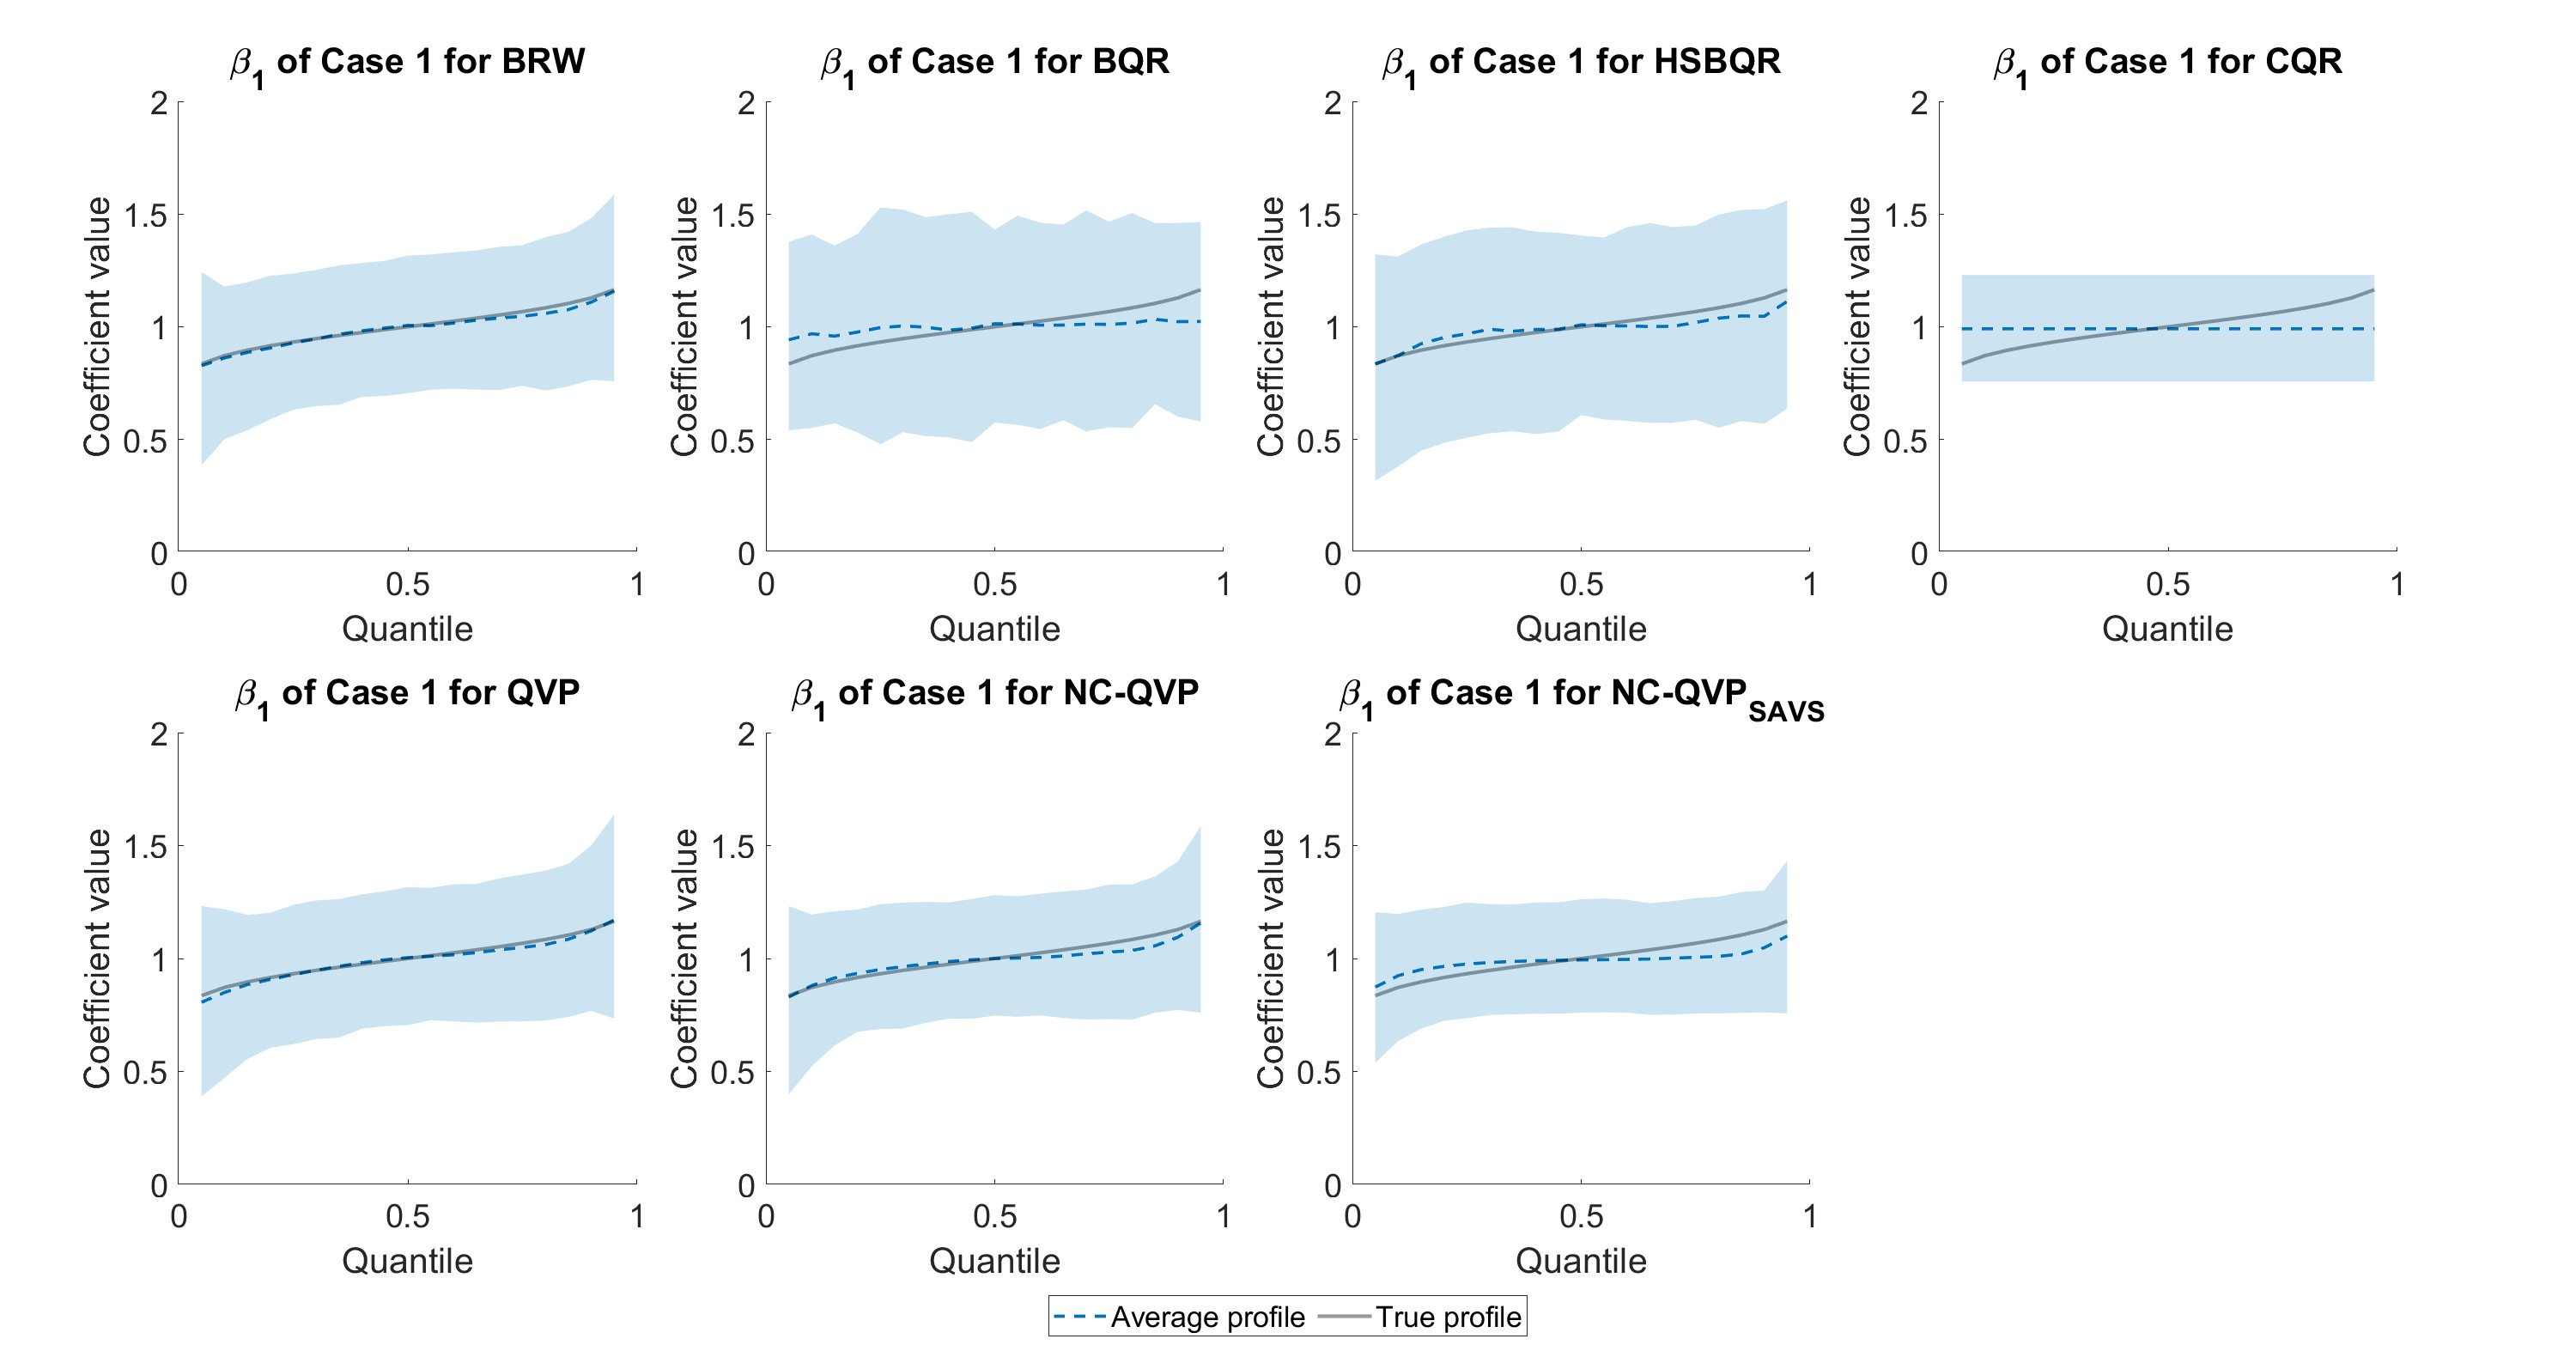
\includegraphics[width=\linewidth]{Figures/PresFig1_T=300.jpg}
    \caption{Quantile varying variable for Case=1, T=300, rho=0.0}
    \label{fig:DGP1}
\end{figure}

%Maybe put this figure to appendix. (fig:\mathrm{DGP}-2)
\begin{figure}[H]
    \centering
    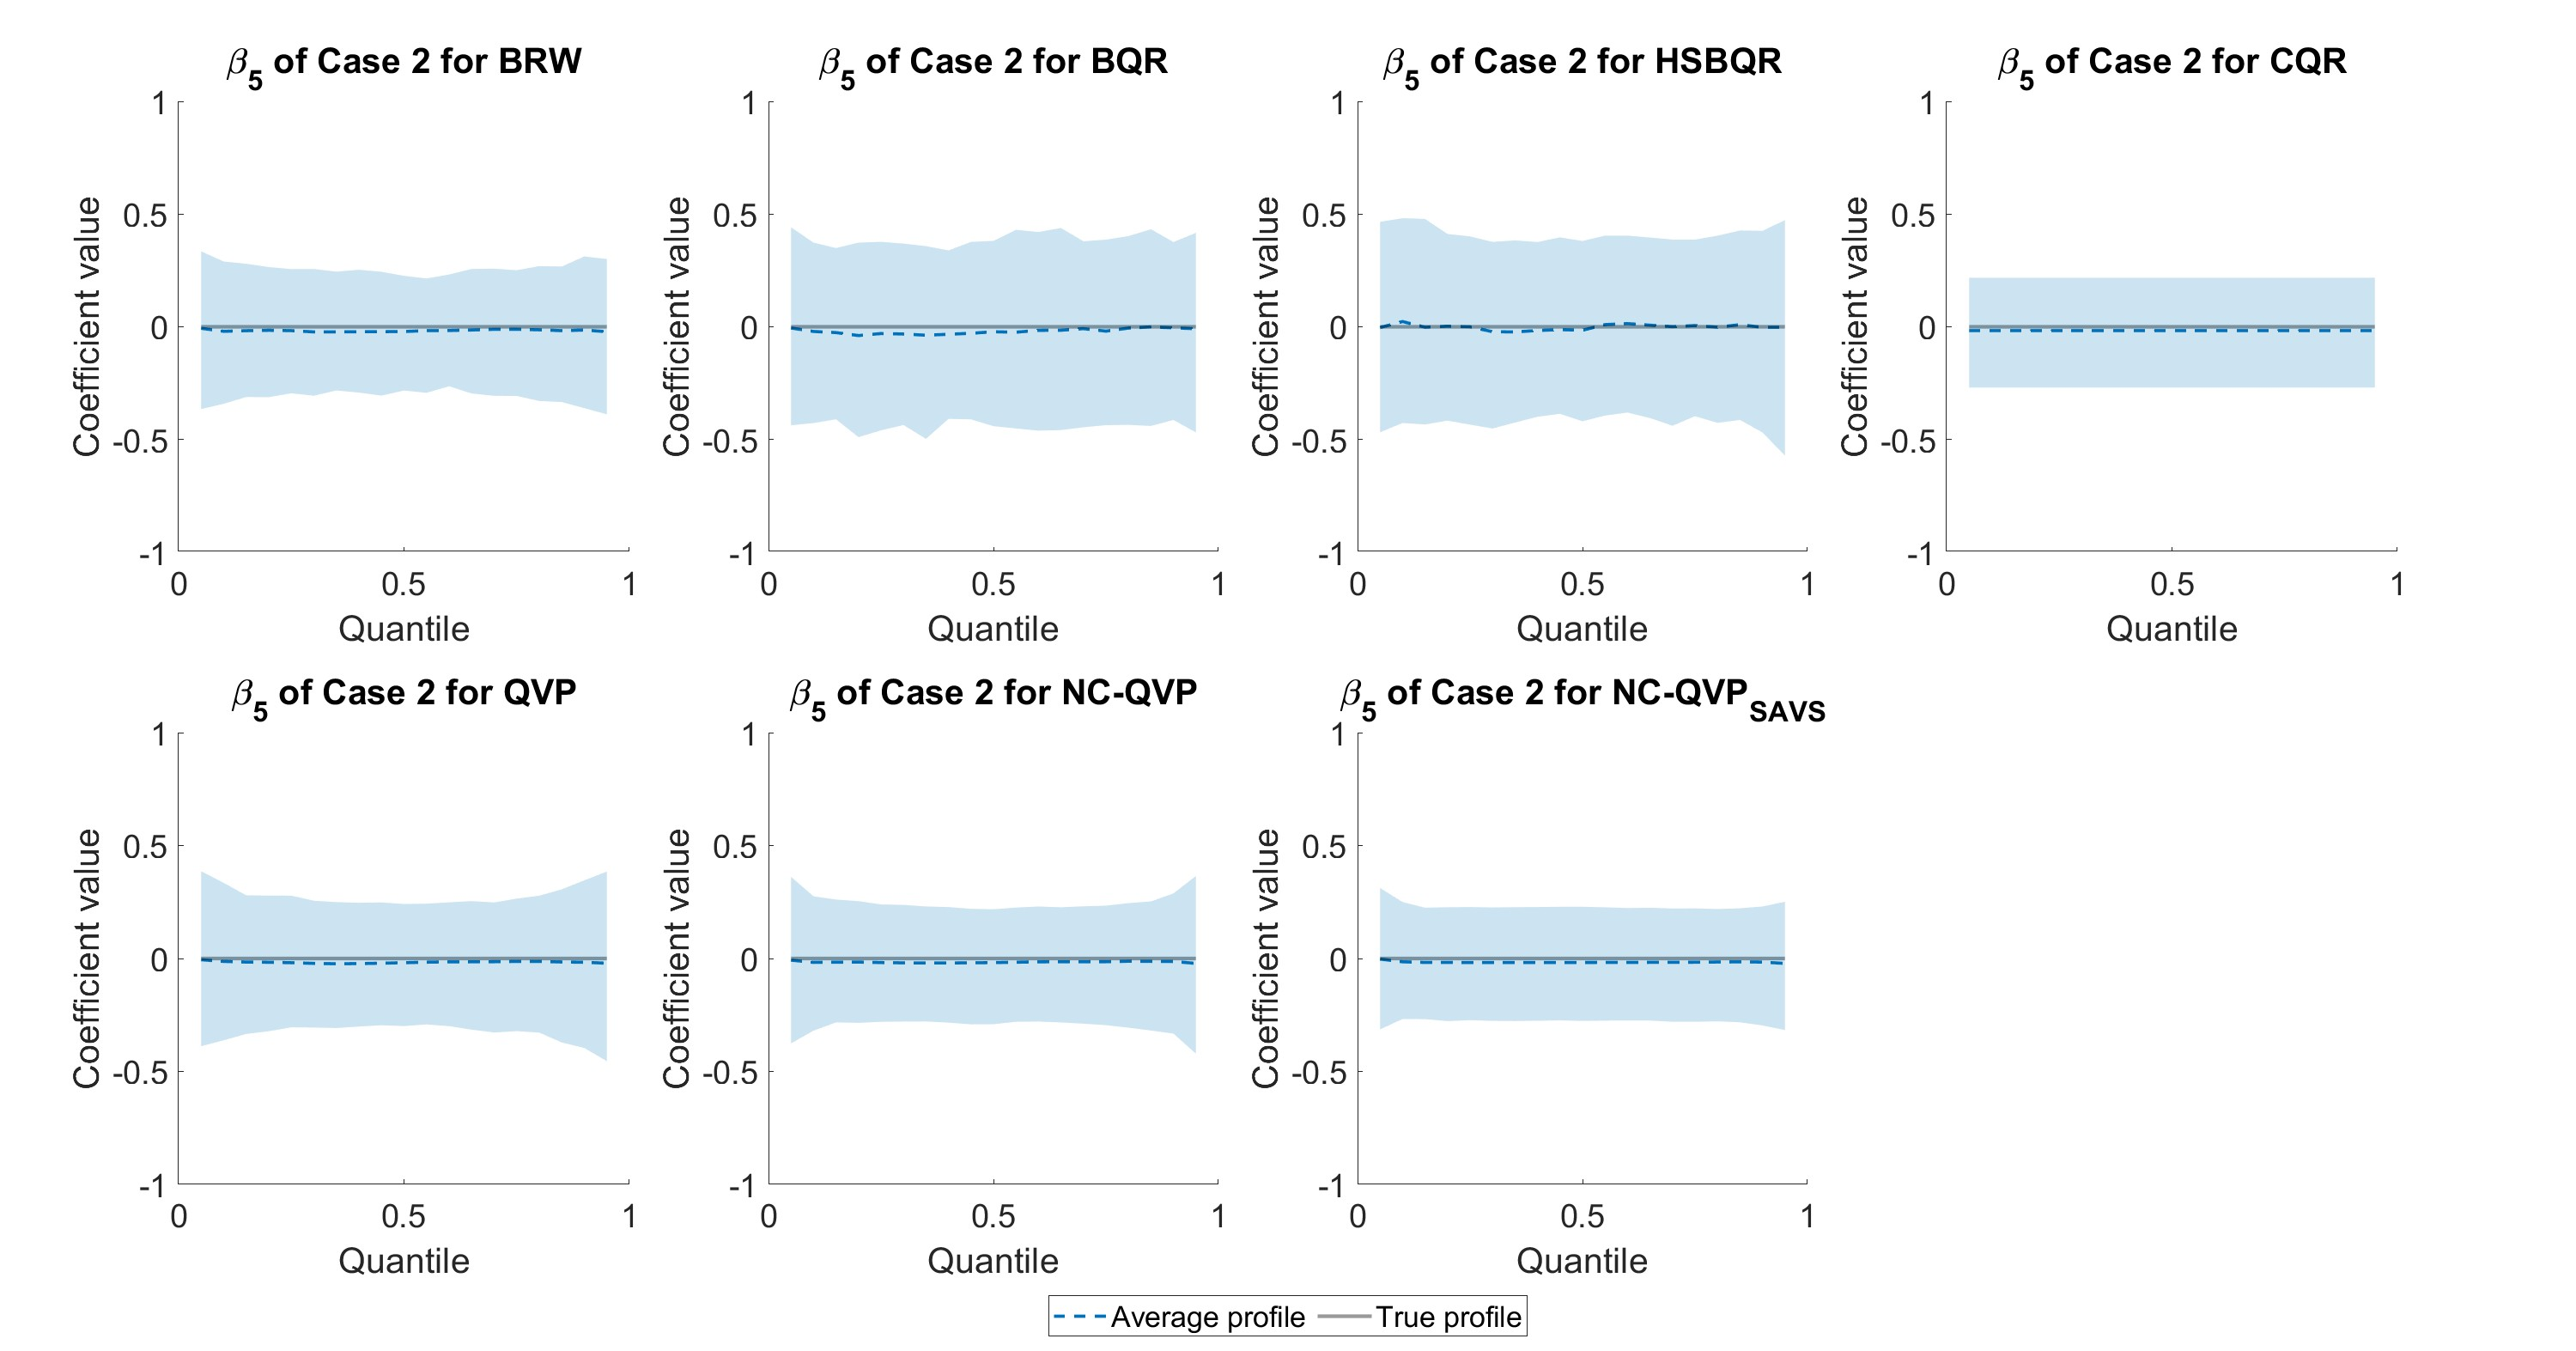
\includegraphics[width=\linewidth]{Figures/PresFig2_T=300.jpg}
    \caption{Quantile constant variable for Case=2, T=300, rho=0.0}
    \label{fig:DGP2}
\end{figure}

%
\begin{figure}[H]
    \centering
    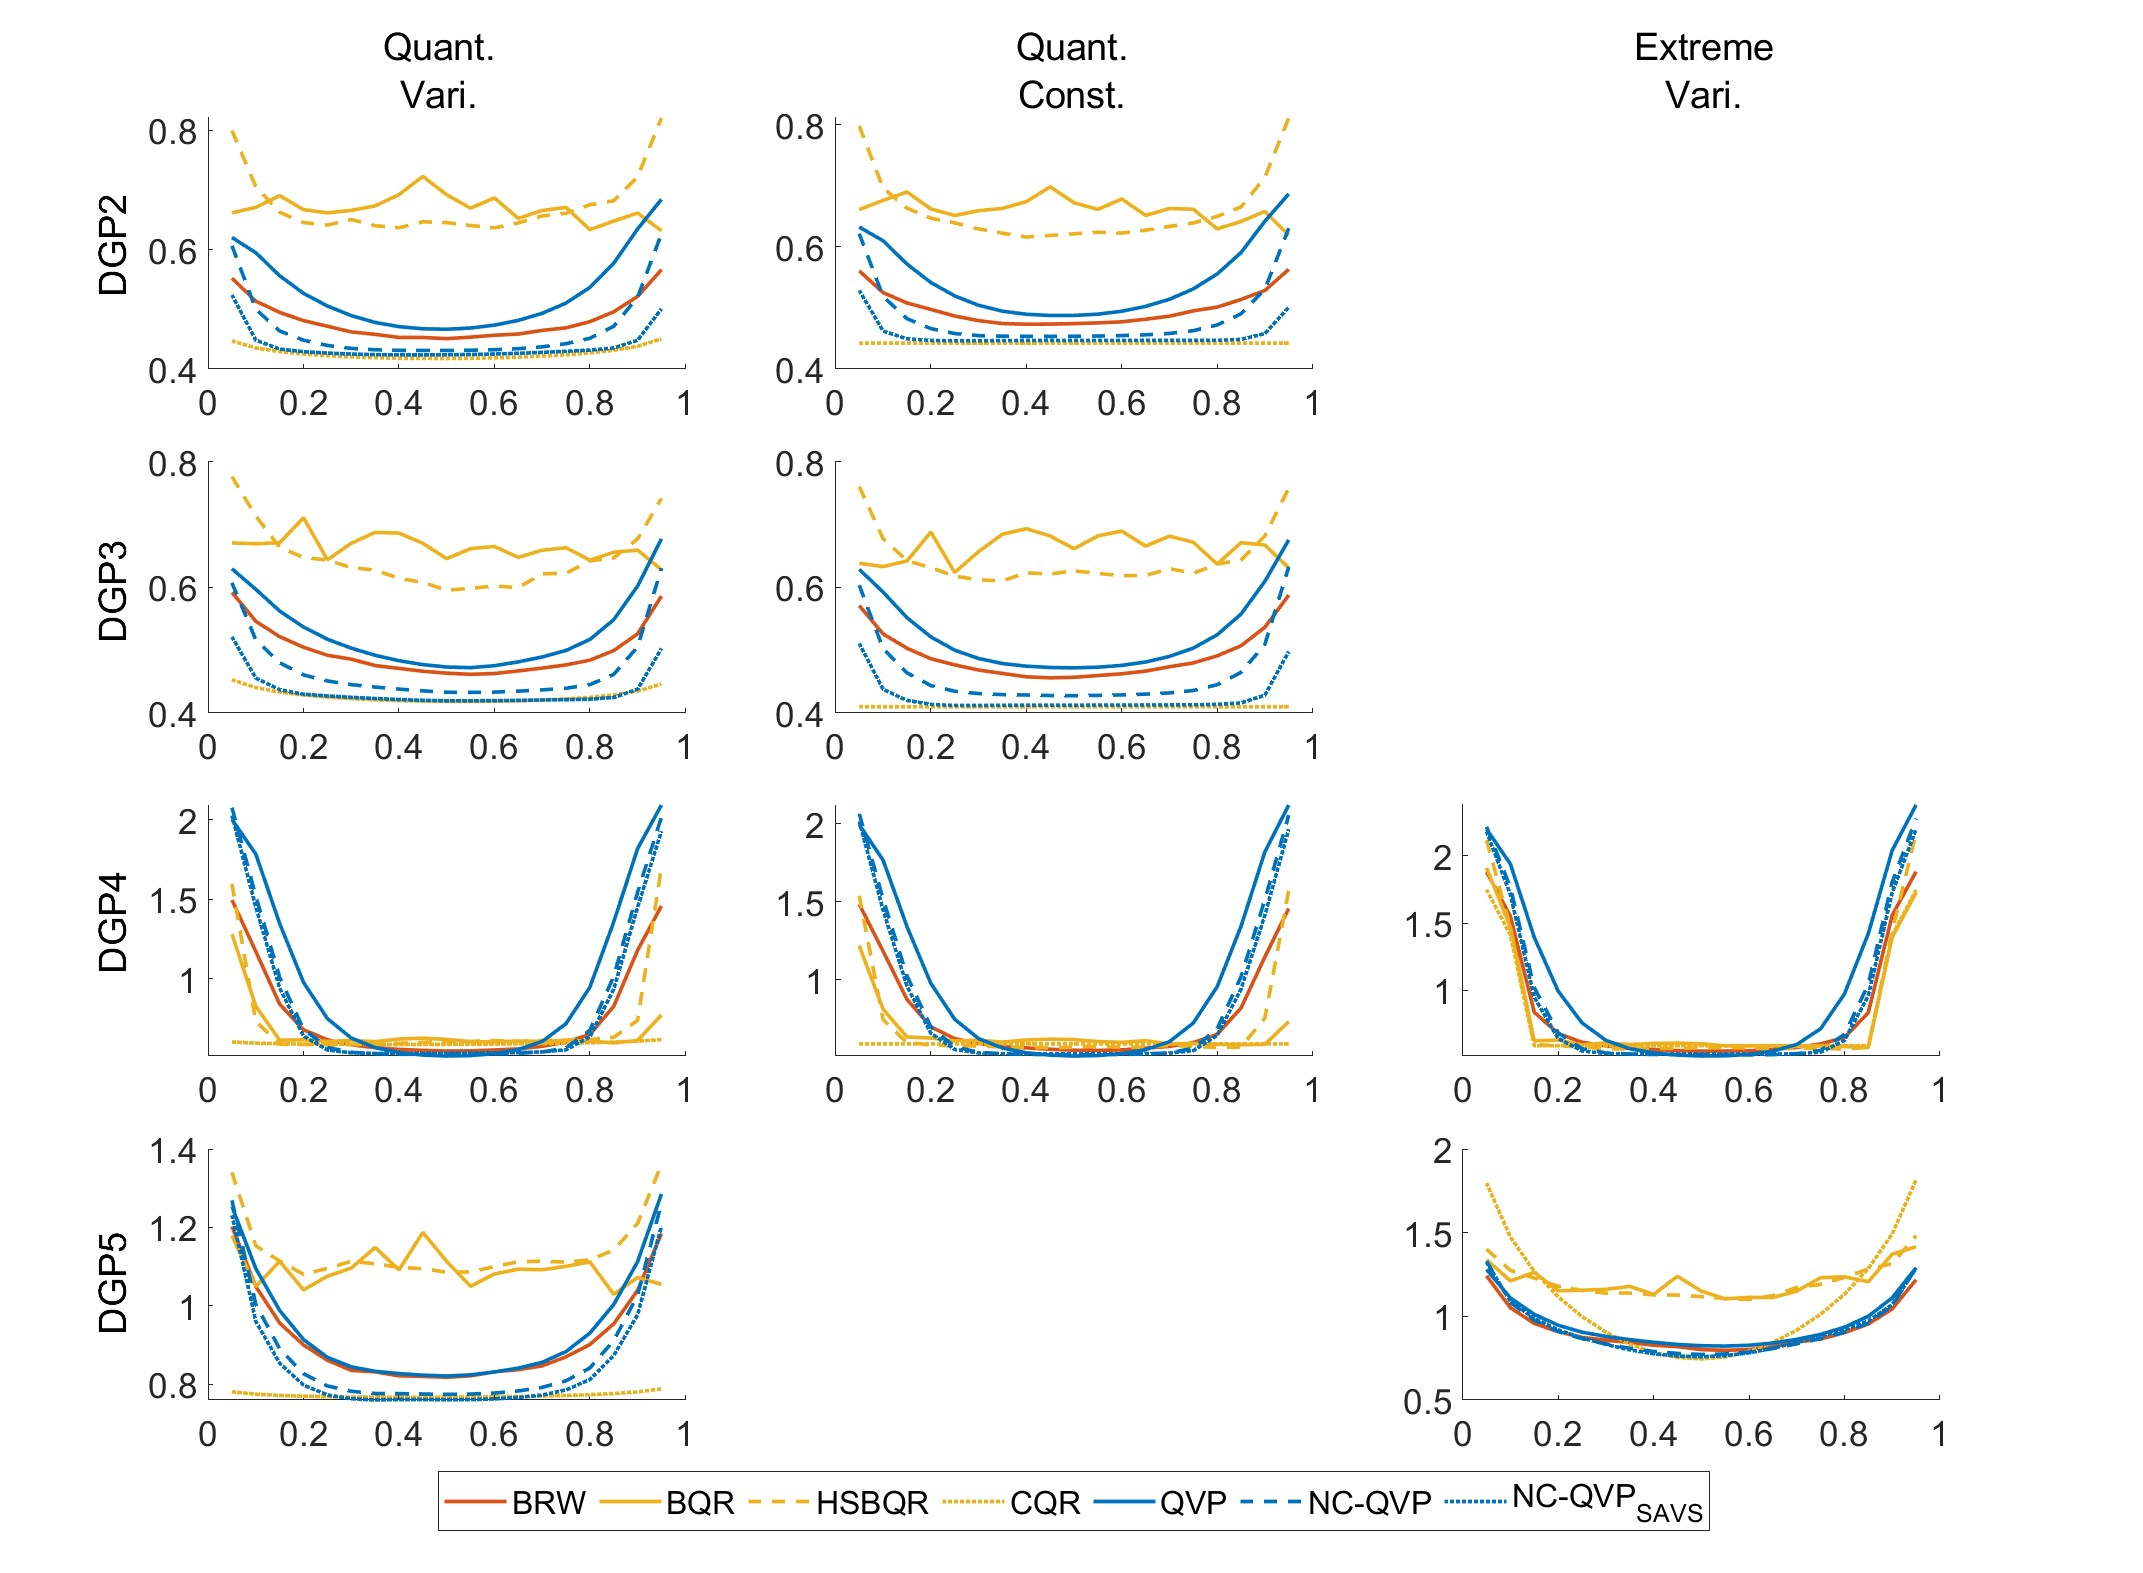
\includegraphics[width=0.9\linewidth]{AppFig/CoeffBiasSpecificv3_T100.jpg}
    \caption{$\rmse$ profile of $\boldsymbol{\beta}$ across 19 quantiles $\tau_q \in \left\{0.05,\dotsc,0.95\right\}$ for $\mathcal{T}=100$ and $\varDelta$=0. Estimates are based on the posterior mean.}
    \label{fig:SpecCoeffBias_T100}
\end{figure}

\begin{figure}[H]
    \centering
    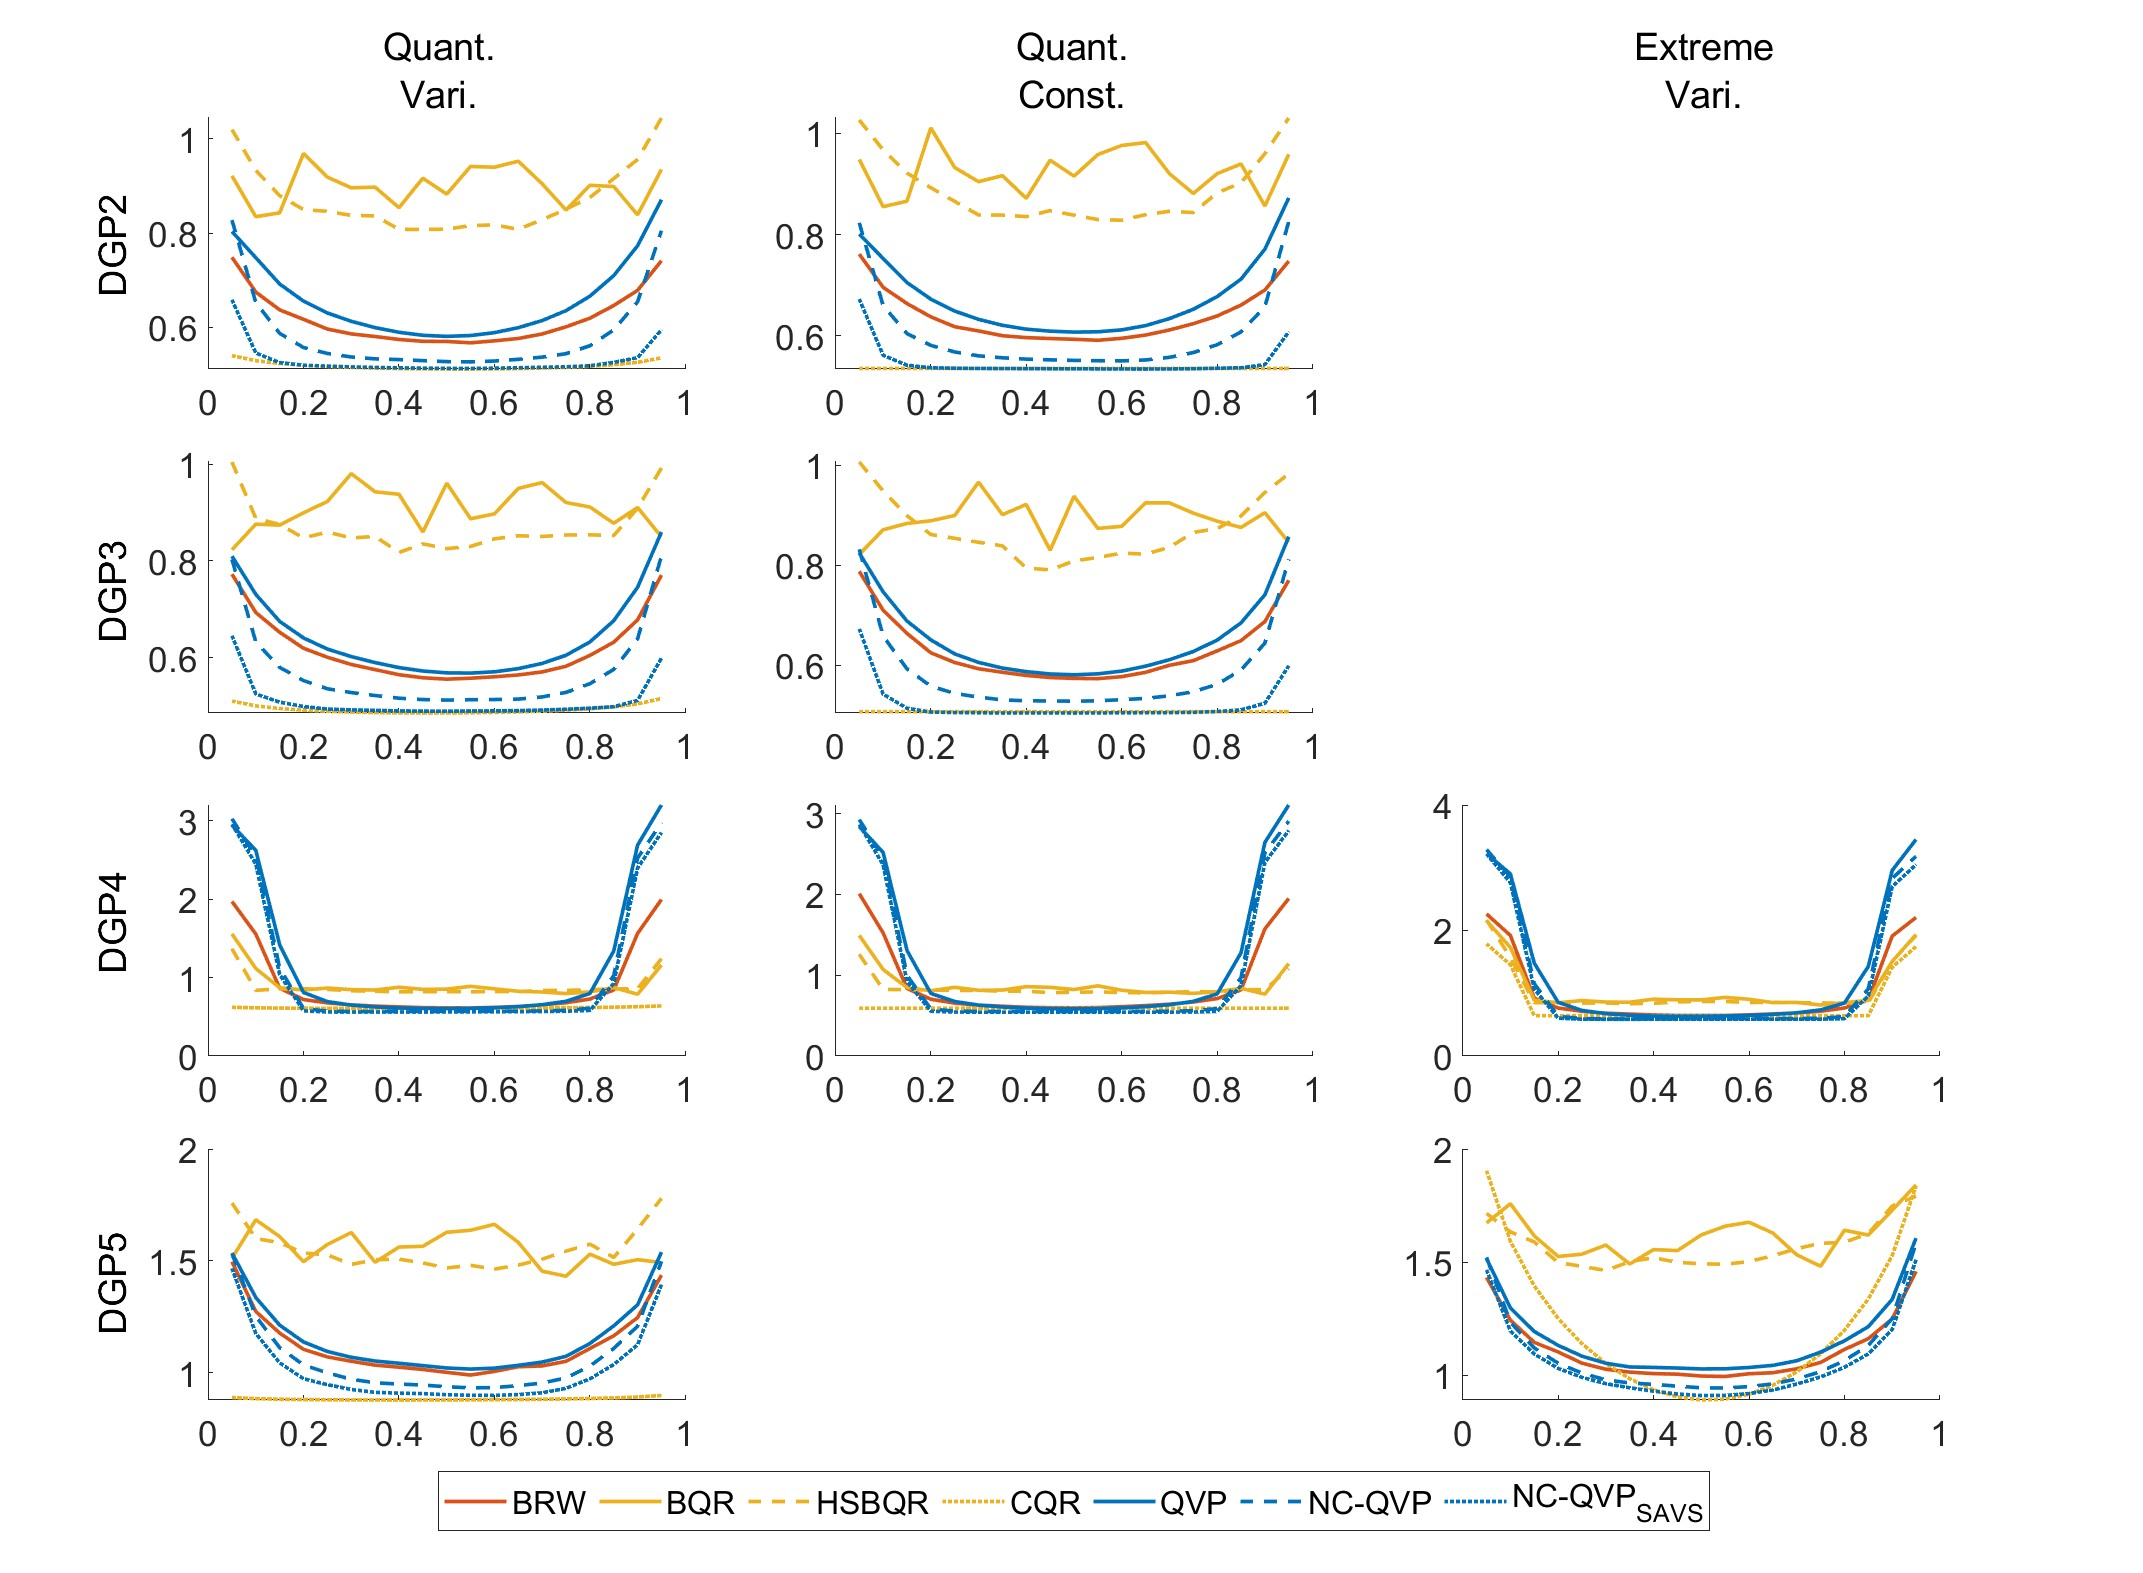
\includegraphics[width=0.9\linewidth]{AppFig/CoeffBiasSpecificv3_rho05.jpg}
    \caption{$\rmse$ profile of $\boldsymbol{\beta}$ across 19 quantiles $\tau_q \in \left\{0.05,\dotsc,0.95\right\}$ for $\mathcal{T}=300$ and $\varDelta$=0.5. Estimates are based on the posterior mean.}
    \label{fig:SpecCoeffBias_rho05}
\end{figure}

\begin{figure}[H]
    \centering
    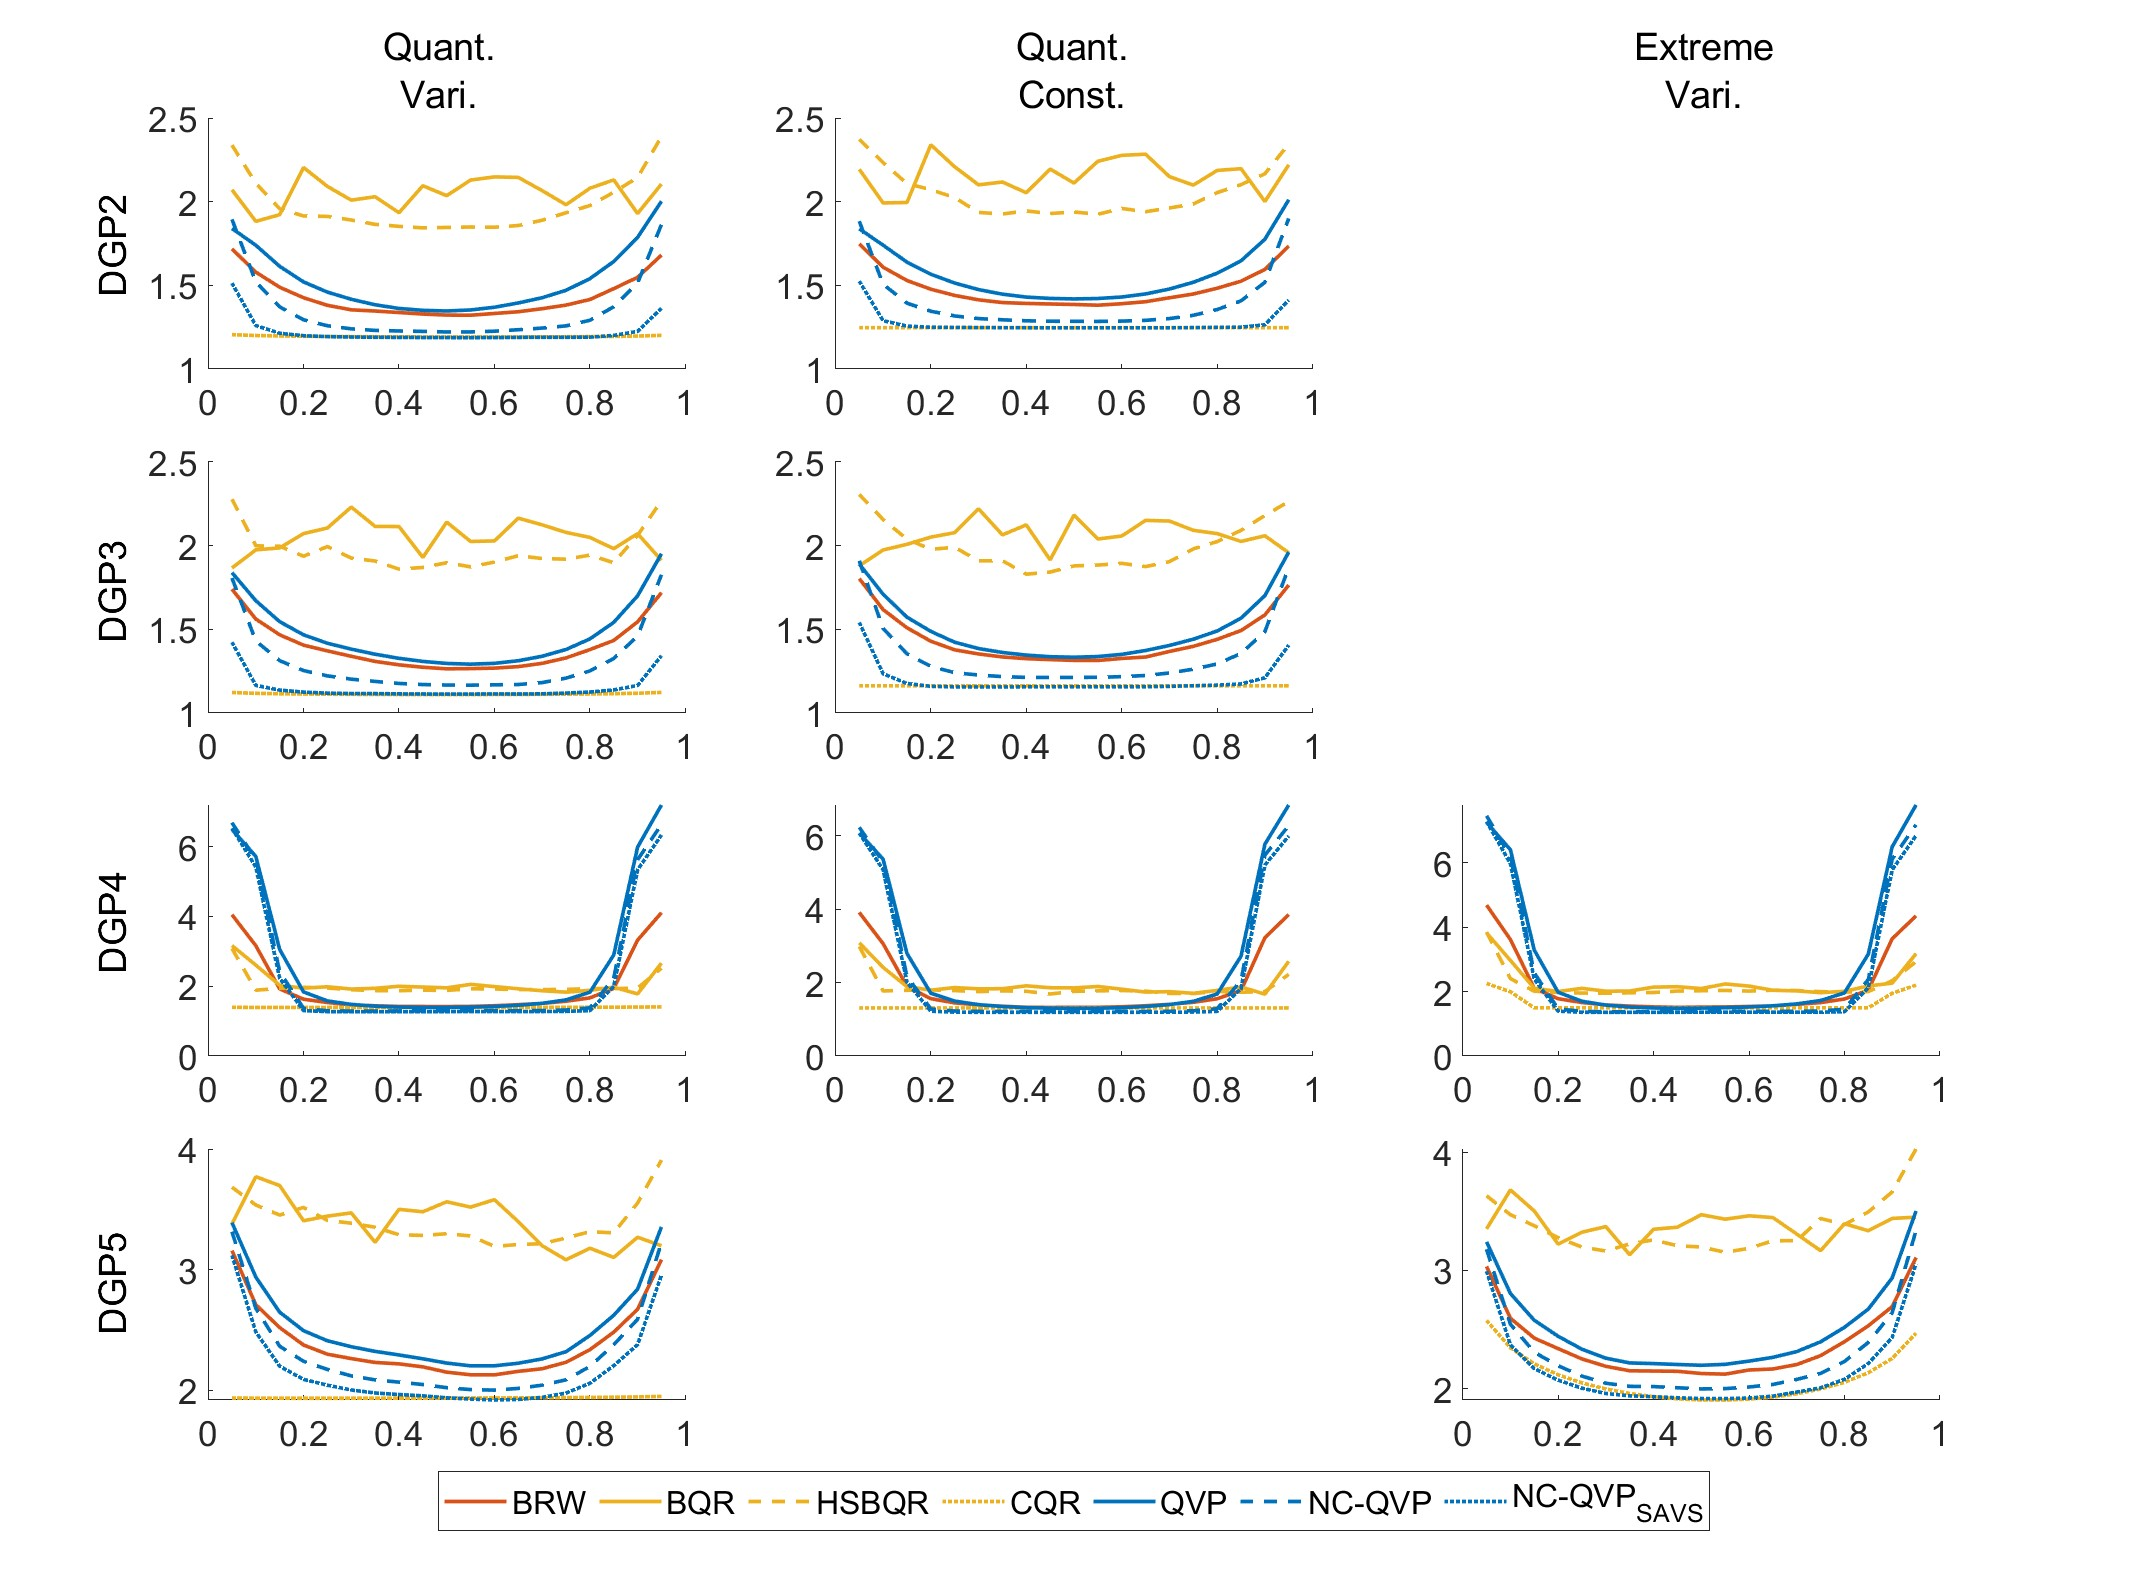
\includegraphics[width=0.9\linewidth]{AppFig/CoeffBiasSpecificv3_rho09.jpg}
    \caption{$\rmse$ profile of $\boldsymbol{\beta}$ across 19 quantiles $\tau_q \in \left\{0.05,\dotsc,0.95\right\}$ for $\mathcal{T}=300$ and $\varDelta$=0.9. Estimates are based on the posterior mean.}
    \label{fig:SpecCoeffBias_rho09}
\end{figure}

\begin{figure}[H]
    \centering
    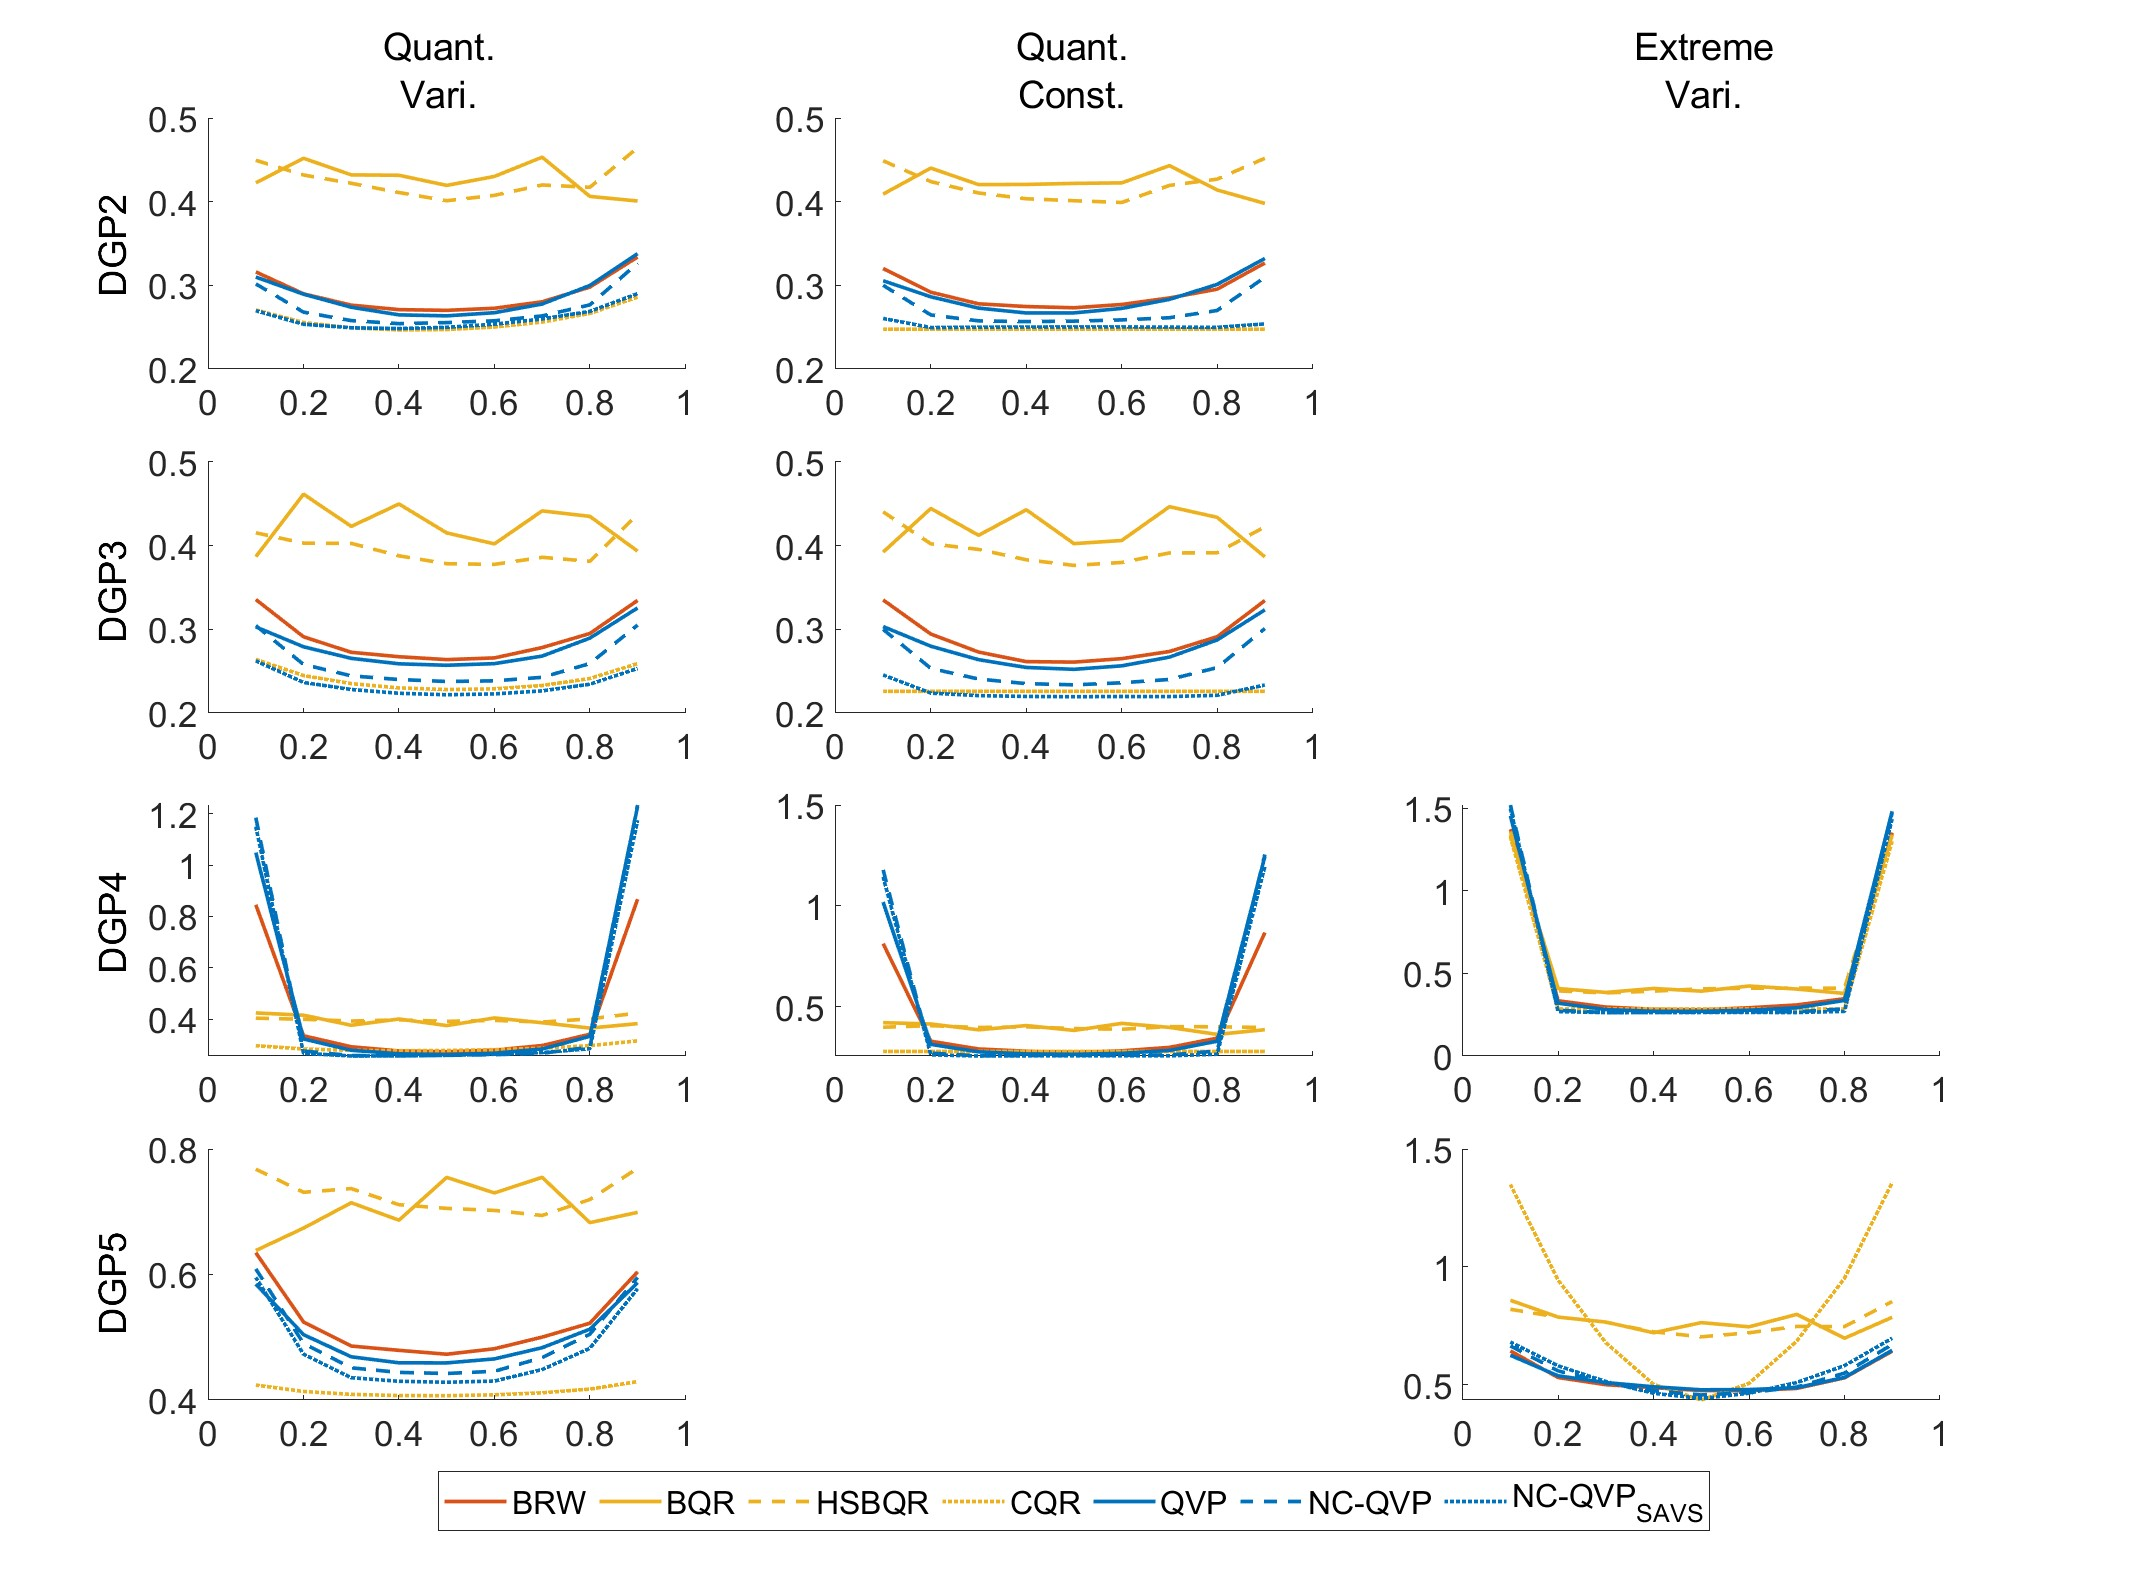
\includegraphics[width=0.9\linewidth]{AppFig/CoeffBiasSpecificv3_Q9.jpg}
    \caption{$\rmse$ profile of $\boldsymbol{\beta}$ across 9 quantiles $\tau_q \in \left\{0.1,\dotsc,0.9\right\}$ for $\mathcal{T}=300$ and $\varDelta$=0. Estimates are based on the posterior mean.}
    \label{fig:SpecCoeffBias_Q9}
\end{figure}

\begin{figure}[H]
    \centering
    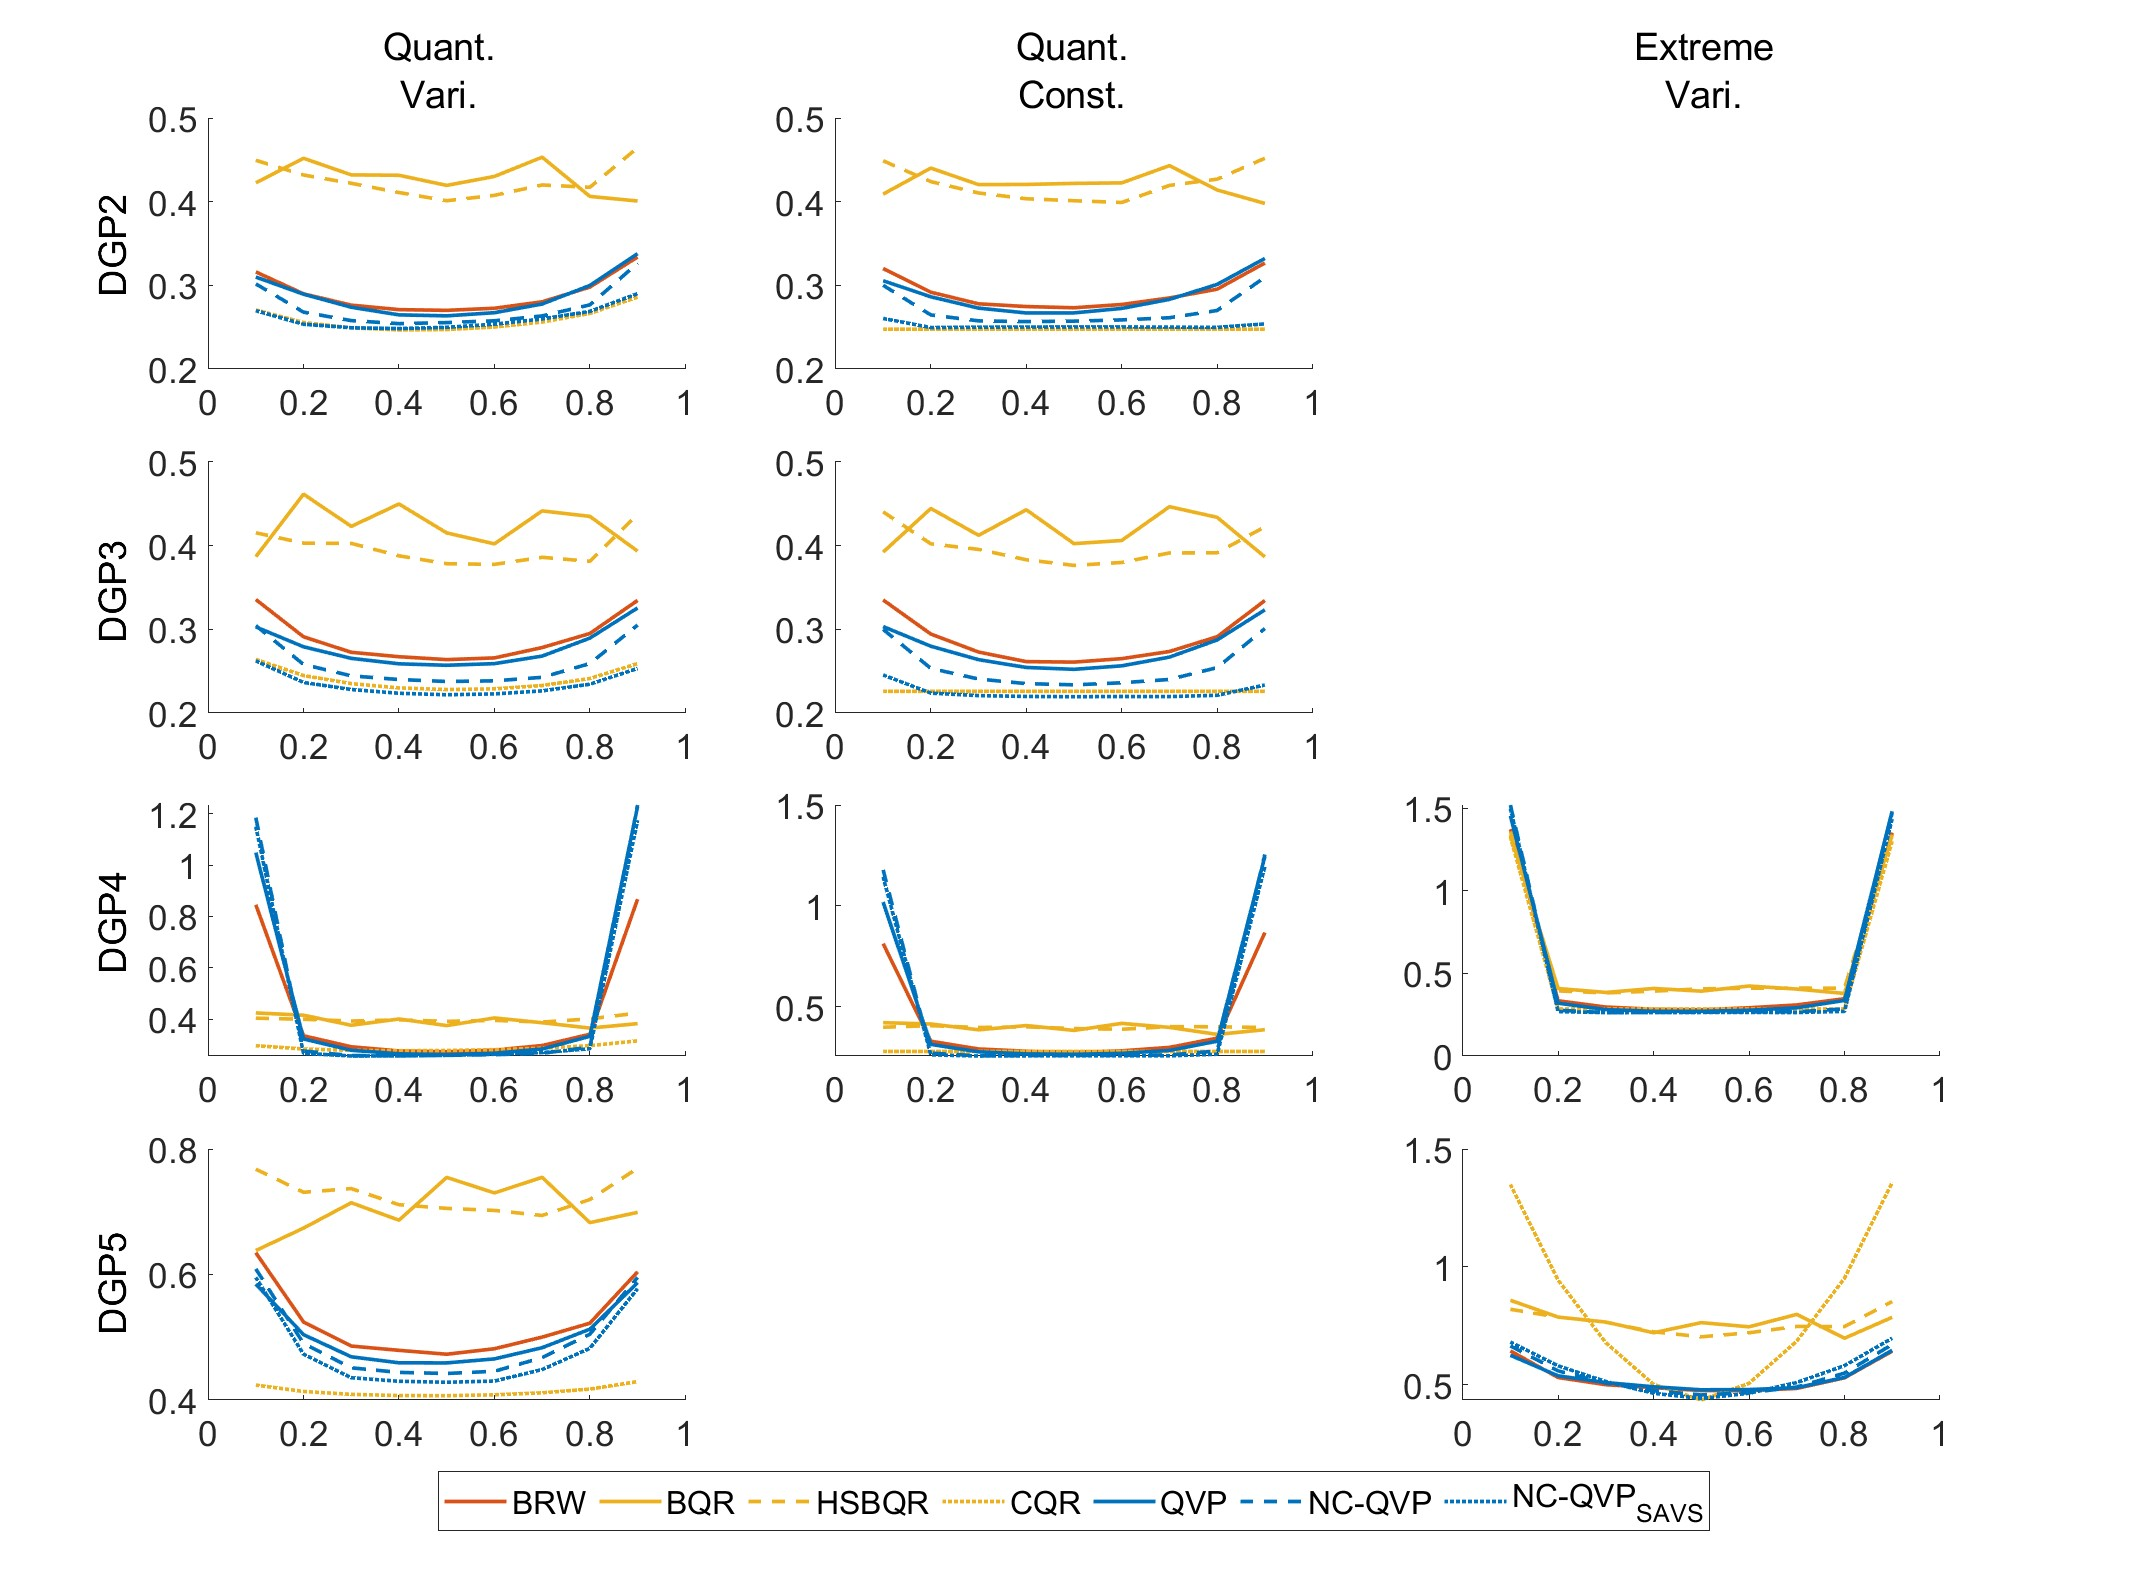
\includegraphics[width=0.9\linewidth]{AppFig/CoeffBiasSpecificv3_Q9.jpg}
    \caption{$\rmse$ profile of $\boldsymbol{\beta}$ across 39 quantiles $\tau_q \in \left\{0.025,\dotsc,0.975\right\}$ for $\mathcal{T}=300$ and $\varDelta$=0. Estimates are based on the posterior mean.}
    \label{fig:SpecCoeffBias_Q39}
\end{figure}

\subsection{Predictive Results}\label{app:sims-predictive-results}
\clearpage

\begin{table}[H]
\centering
\resizebox{0.9\textwidth}{!}{%
\begin{tabular}{ll|cccc|cccc}
 &  & \multicolumn{4}{c|}{$\varDelta$=0.5} & \multicolumn{4}{c}{$\varDelta$=0.9} \\
 &  & $w_1$ & $w_2$ & $w_3$ & $w_4$ & $w_1$ & $w_2$ & $w_3$ & $w_4$ \\ \hline
\multicolumn{2}{l|}{$\mathrm{DGP}$-1} &  &  &  &  &  &  \\
 & $\BQR$   & 0.421 & 0.078 & 0.132 & 0.133 & 0.420 & 0.078 & 0.132 & 0.133 \\ \hdashline
 & $\HSBQR$ & 0.911 & 0.950 & 0.892 & 0.883 & 0.912 & 0.949 & 0.892 & 0.881 \\
 & $\BRW$   & 0.855 & 0.906 & 0.828 & 0.821 & 0.856 & 0.905 & 0.827 & 0.82 \\
 & $\CQR$   & 0.852 & 0.904 & 0.824 & 0.818 & 0.853 & 0.903 & 0.823 & 0.817 \\
 & $\QVP$   & 0.854 & 0.906 & 0.828 & 0.820 & 0.856 & 0.905 & 0.827 & 0.819 \\
 & $\NCQVP$ & 0.853 & 0.905 & 0.826 & 0.819 & 0.854 & 0.904 & 0.825 & 0.818 \\
 & $\NCQVP_{\mathrm{SAVS}}$ & 0.852 & 0.904 & 0.825 & 0.818 & 0.853 & 0.903 & 0.823 & 0.817 \\ \hline
\multicolumn{2}{l|}{$\mathrm{DGP}$-2} &  &  &  &  &  &  \\
 & $\BQR$   & 0.433 & 0.080 & 0.134 & 0.138 & 0.433 & 0.08 & 0.134 & 0.138 \\ \hdashline
 & $\HSBQR$ & 0.908 & 0.949 & 0.897 & 0.878 & 0.907 & 0.948 & 0.896 & 0.877 \\
 & $\BRW$   & 0.842 & 0.895 & 0.825 & 0.802 & 0.841 & 0.895 & 0.824 & 0.801 \\
 & $\CQR$   & 0.837 & 0.891 & 0.819 & 0.797 & 0.836 & 0.890 & 0.819 & 0.797 \\
 & $\QVP$   & 0.843 & 0.897 & 0.826 & 0.805 & 0.843 & 0.896 & 0.826 & 0.804 \\
 & $\NCQVP$ & 0.839 & 0.892 & 0.822 & 0.800 & 0.839 & 0.892 & 0.822 & 0.799 \\
 & $\NCQVP_{\mathrm{SAVS}}$ & 0.837 & 0.891 & 0.820 & 0.797 & 0.836 & 0.890 & 0.820 & 0.797 \\ \hline
\multicolumn{2}{l|}{$\mathrm{DGP}$-3} &  &  &  &  &  &  \\
 & $\BQR$   & 0.412 & 0.076 & 0.132 & 0.128 & 0.412 & 0.076 & 0.132 & 0.128 \\ \hdashline
 & $\HSBQR$ & 0.906 & 0.948 & 0.867 & 0.895 & 0.906 & 0.949 & 0.867 & 0.896 \\
 & $\BRW$   & 0.844 & 0.899 & 0.800 & 0.823 & 0.844 & 0.899 & 0.800 & 0.824 \\
 & $\CQR$   & 0.840 & 0.895 & 0.796 & 0.819 & 0.840 & 0.896 & 0.796 & 0.819 \\
 & $\QVP$   & 0.844 & 0.899 & 0.800 & 0.824 & 0.844 & 0.900 & 0.801 & 0.824 \\
 & $\NCQVP$ & 0.841 & 0.896 & 0.798 & 0.821 & 0.842 & 0.897 & 0.798 & 0.821 \\
 & $\NCQVP_{\mathrm{SAVS}}$ & 0.840 & 0.895 & 0.796 & 0.819 & 0.840 & 0.895 & 0.796 & 0.819 \\ \hline
\multicolumn{2}{l|}{$\mathrm{DGP}$-4} &  &  &  &  &  &  \\
 & $\BQR$   & 0.779 & 0.141 & 0.245 & 0.251 & 0.779 & 0.141 & 0.245 & 0.251 \\ \hdashline
 & $\HSBQR$ & 0.996 & 0.998 & 1.006 & 0.987 & 0.995 & 0.997 & 1.005 & 0.986 \\
 & $\BRW$   & 0.903 & 0.941 & 0.893 & 0.873 & 0.902 & 0.941 & 0.892 & 0.872 \\
 & $\CQR$   & 0.901 & 0.940 & 0.891 & 0.871 & 0.902 & 0.940 & 0.892 & 0.871 \\
 & $\QVP$   & 0.906 & 0.943 & 0.897 & 0.878 & 0.906 & 0.943 & 0.897 & 0.877 \\
 & $\NCQVP$ & 0.903 & 0.940 & 0.894 & 0.874 & 0.903 & 0.939 & 0.894 & 0.873 \\
 & $\NCQVP_{\mathrm{SAVS}}$ & 0.903 & 0.940 & 0.894 & 0.873 & 0.902 & 0.939 & 0.893 & 0.872 \\ \hline
\multicolumn{2}{l|}{$\mathrm{DGP}$-5} &  &  &  &  &  &  \\
 & $\BQR$   & 0.720 & 0.134 & 0.221 & 0.230 & 0.717 & 0.134 & 0.220 & 0.229 \\ \hdashline
 & $\HSBQR$ & 0.935 & 0.971 & 0.933 & 0.899 & 0.936 & 0.968 & 0.934 & 0.900 \\
 & $\BRW$   & 0.879 & 0.927 & 0.868 & 0.836 & 0.880 & 0.925 & 0.870 & 0.837 \\
 & $\CQR$   & 0.880 & 0.928 & 0.871 & 0.837 & 0.883 & 0.927 & 0.874 & 0.841 \\
 & $\QVP$   & 0.879 & 0.928 & 0.868 & 0.836 & 0.880 & 0.925 & 0.870 & 0.837 \\
 & $\NCQVP$ & 0.878 & 0.927 & 0.868 & 0.835 & 0.879 & 0.924 & 0.869 & 0.836 \\
 & $\NCQVP_{\mathrm{SAVS}}$ & 0.878 & 0.926 & 0.867 & 0.835 & 0.879 & 0.924 & 0.869 & 0.836 \\ \hline
\end{tabular}%
}
\caption{Out-of-sample predictive performance for $\mathcal{T}=300$ as measured by the weighted quantile score, $\mathrm{qwQS}$, see Equation~\ref{eq:qwQS}. Weighting schemes are $w_{q} = 1/\mathcal{Q}$ ($\QS$) which is equal to the $\mathrm{CRPS}$. $w_{q} = \tau_q(1-\tau_q)$ (Centre) places more weight the central quantiles, $w_{q} = (1-\tau_q)^2$ (Left) places more weight on left tail quantiles, $w_{\tau_q} = \tau^2_q$ (Right) places more weight on right tail quantiles. Performance is shown relative to $\BQR$ whose absolute performance shown above the dotted lines respectively.}
\label{tab:overallbias_main_correlation}
\end{table}
\begin{table}[H]
\centering
\resizebox{0.9\textwidth}{!}{%
\begin{tabular}{ll|cccc|cccc}
 &  & \multicolumn{4}{c|}{$\mathcal{Q}=9$} & \multicolumn{4}{c}{$\mathcal{Q}=39$} \\
 &  & $w_1$ & $w_2$ & $w_3$ & $w_4$ & $w_1$ & $w_2$ & $w_3$ & $w_4$ \\ \hline
\multicolumn{2}{l|}{$\mathrm{DGP}$-1} &  &  &  &  &  &  \\
 & $\BQR$   & 0.446 & 0.084 & 0.136 & 0.142 & 0.418 & 0.076 & 0.131 & 0.135 \\ \hdashline
 & $\HSBQR$ & 0.901 & 0.937 & 0.900 & 0.859 & 0.904 & 0.957 & 0.888 & 0.859 \\
 & $\BRW$   & 0.847 & 0.893 & 0.837 & 0.801 & 0.846 & 0.912 & 0.821 & 0.797 \\
 & $\CQR$   & 0.843 & 0.890 & 0.833 & 0.798 & 0.843 & 0.909 & 0.818 & 0.793 \\
 & $\QVP$   & 0.846 & 0.892 & 0.835 & 0.800 & 0.846 & 0.912 & 0.821 & 0.797 \\
 & $\NCQVP$ & 0.845 & 0.891 & 0.835 & 0.799 & 0.844 & 0.910 & 0.820 & 0.795 \\
 & $\NCQVP_{\mathrm{SAVS}}$ & 0.843 & 0.890 & 0.833 & 0.798 & 0.843 & 0.909 & 0.818 & 0.793 \\ \hline
\multicolumn{2}{l|}{$\mathrm{DGP}$-2} &  &  &  &  &  &  \\
 & $\BQR$   & 0.439 & 0.084 & 0.136 & 0.135 & 0.421 & 0.077 & 0.134 & 0.133 \\ \hdashline
 & $\HSBQR$ & 0.932 & 0.953 & 0.913 & 0.926 & 0.915 & 0.961 & 0.881 & 0.895 \\
 & $\BRW$   & 0.865 & 0.898 & 0.840 & 0.849 & 0.844 & 0.904 & 0.806 & 0.814 \\
 & $\CQR$   & 0.860 & 0.894 & 0.835 & 0.844 & 0.840 & 0.900 & 0.800 & 0.809 \\
 & $\QVP$   & 0.864 & 0.897 & 0.839 & 0.848 & 0.848 & 0.907 & 0.810 & 0.818 \\
 & $\NCQVP$ & 0.862 & 0.895 & 0.837 & 0.846 & 0.843 & 0.902 & 0.804 & 0.813 \\
 & $\NCQVP_{\mathrm{SAVS}}$ & 0.860 & 0.894 & 0.835 & 0.844 & 0.841 & 0.901 & 0.801 & 0.810 \\ \hline
\multicolumn{2}{l|}{$\mathrm{DGP}$-3} &  &  &  &  &  &  \\
 & $\BQR$   & 0.420 & 0.080 & 0.126 & 0.134 & 0.409 & 0.074 & 0.131 & 0.130 \\ \hdashline
 & $\HSBQR$ & 0.924 & 0.950 & 0.937 & 0.882 & 0.892 & 0.949 & 0.858 & 0.863 \\
 & $\BRW$   & 0.864 & 0.901 & 0.868 & 0.815 & 0.831 & 0.899 & 0.79 & 0.794 \\
 & $\CQR$   & 0.859 & 0.896 & 0.863 & 0.810 & 0.827 & 0.896 & 0.786 & 0.790 \\
 & $\QVP$   & 0.862 & 0.899 & 0.867 & 0.814 & 0.832 & 0.900 & 0.792 & 0.796 \\
 & $\NCQVP$ & 0.860 & 0.897 & 0.865 & 0.812 & 0.829 & 0.897 & 0.788 & 0.792 \\
 & $\NCQVP_{\mathrm{SAVS}}$ & 0.858 & 0.896 & 0.863 & 0.810 & 0.827 & 0.896 & 0.786 & 0.790 \\ \hline
\multicolumn{2}{l|}{$\mathrm{DGP}$-4} &  &  &  &  &  &  \\
 & $\BQR$   & 0.790 & 0.148 & 0.244 & 0.249 & 0.770 & 0.138 & 0.245 & 0.249 \\ \hdashline
 & $\HSBQR$ & 0.997 & 1.000 & 1.004 & 0.992 & 0.986 & 0.993 & 0.986 & 0.979 \\
 & $\BRW$   & 0.929 & 0.948 & 0.927 & 0.912 & 0.895 & 0.937 & 0.876 & 0.866 \\
 & $\CQR$   & 0.927 & 0.947 & 0.924 & 0.909 & 0.893 & 0.937 & 0.875 & 0.863 \\
 & $\QVP$   & 0.929 & 0.948 & 0.926 & 0.913 & 0.902 & 0.941 & 0.885 & 0.875 \\
 & $\NCQVP$ & 0.928 & 0.946 & 0.926 & 0.911 & 0.897 & 0.937 & 0.88 & 0.869 \\
 & $\NCQVP_{\mathrm{SAVS}}$ & 0.927 & 0.946 & 0.925 & 0.910 & 0.896 & 0.937 & 0.879 & 0.868 \\ \hline
\multicolumn{2}{l|}{$\mathrm{DGP}$-5} &  &  &  &  &  &  \\
 & $\BQR$   & 0.709 & 0.138 & 0.218 & 0.214 & 0.708 & 0.130 & 0.222 & 0.226 \\ \hdashline
 & $\HSBQR$ & 0.985 & 0.990 & 0.971 & 0.996 & 0.926 & 0.971 & 0.906 & 0.894 \\
 & $\BRW$   & 0.927 & 0.947 & 0.909 & 0.926 & 0.869 & 0.927 & 0.843 & 0.828 \\
 & $\CQR$   & 0.931 & 0.949 & 0.914 & 0.931 & 0.874 & 0.930 & 0.849 & 0.834 \\
 & $\QVP$   & 0.927 & 0.946 & 0.908 & 0.925 & 0.870 & 0.928 & 0.844 & 0.829 \\
 & $\NCQVP$ & 0.926 & 0.946 & 0.908 & 0.925 & 0.869 & 0.927 & 0.843 & 0.828 \\
 & $\NCQVP_{\mathrm{SAVS}}$ & 0.926 & 0.945 & 0.908 & 0.925 & 0.869 & 0.927 & 0.843 & 0.828 \\ \hline
\end{tabular}%
}
\caption{Out-of-sample predictive performance for $\mathcal{T}=300$ as measured by the weighted quantile score, $\mathrm{qwQS}$, see Equation~\ref{eq:qwQS}. Weighting schemes are $w_{q} = 1/\mathcal{Q}$ ($\QS$) which is equal to the $\mathrm{CRPS}$. $w_{q} = \tau_q(1-\tau_q)$ (Centre) places more weight the central quantiles, $w_{q} = (1-\tau_q)^2$ (Left) places more weight on left tail quantiles, $w_{\tau_q} = \tau^2_q$ (Right) places more weight on right tail quantiles. Performance is shown relative to $\BQR$ whose absolute performance shown above the dotted lines respectively.}
\label{tab:overallbias_quant}
\end{table}

% Prediction results
\begin{table}[H]
\centering
\resizebox{0.9\textwidth}{!}{%
\begin{tabular}{ll|cccc|cccc}
 &  & \multicolumn{4}{c|}{$\mathcal{T}$=300} & \multicolumn{4}{c}{$\mathcal{T}$=100} \\
 &  & $w_1$ & $w_2$ & $w_3$ & $w_4$ & $w_1$ & $w_2$ & $w_3$ & $w_4$ \\ \hline
\multicolumn{2}{l|}{$\mathrm{DGP}$-1} &  &  &  &  &  &  \\
 & $\BQR$ & 0.424 & 0.078 & 0.133 & 0.134 & 0.438 & 0.081 & 0.137 & 0.138 \\ \hdashline
 & $\HSBQR$ & 0.911 & 0.957 & 0.892 & 0.882 & 0.920 & 0.957 & 0.903 & 0.898 \\
 & $\BRW$ & 0.853 & 0.912 & 0.826 & 0.819 & 0.845 & 0.897 & 0.821 & 0.815 \\
 & $\CQR$ & 0.850 & 0.908 & 0.822 & 0.815 & 0.836 & 0.888 & 0.811 & 0.805 \\
 & $\QVP$ & 0.853 & 0.911 & 0.825 & 0.819 & 0.845 & 0.896 & 0.821 & 0.815 \\
 & $\NCQVP$ & 0.851 & 0.910 & 0.824 & 0.817 & 0.840 & 0.891 & 0.816 & 0.810 \\
 & $\NCQVP_{\mathrm{SAVS}}$ & 0.850 & 0.908 & 0.822 & 0.815 & 0.837 & 0.888 & 0.812 & 0.806 \\ \hline
\multicolumn{2}{l|}{$\mathrm{DGP}$-2} &  &  &  &  &  &  \\
 & $\BQR$ & 0.433 & 0.08 & 0.135 & 0.138 & 0.471 & 0.087 & 0.149 & 0.149 \\ \hdashline
 & $\HSBQR$ & 0.909 & 0.950 & 0.893 & 0.878 & 0.910 & 0.945 & 0.885 & 0.888 \\
 & $\BRW$ & 0.841 & 0.894 & 0.817 & 0.802 & 0.816 & 0.866 & 0.784 & 0.785 \\
 & $\CQR$ & 0.836 & 0.890 & 0.812 & 0.797 & 0.806 & 0.857 & 0.773 & 0.773 \\
 & $\QVP$ & 0.842 & 0.895 & 0.819 & 0.804 & 0.822 & 0.871 & 0.790 & 0.793 \\
 & $\NCQVP$ & 0.839 & 0.892 & 0.815 & 0.800 & 0.811 & 0.860 & 0.779 & 0.78 \\
 & $\NCQVP_{\mathrm{SAVS}}$ & 0.837 & 0.891 & 0.813 & 0.798 & 0.806 & 0.857 & 0.774 & 0.774 \\ \hline
\multicolumn{2}{l|}{$\mathrm{DGP}$-3} &  &  &  &  &  &  \\
 & $\BQR$ & 0.413 & 0.076 & 0.133 & 0.128 & 0.437 & 0.081 & 0.133 & 0.143 \\ \hdashline
 & $\HSBQR$ & 0.906 & 0.950 & 0.864 & 0.896 & 0.905 & 0.938 & 0.915 & 0.851 \\
 & $\BRW$ & 0.843 & 0.900 & 0.796 & 0.825 & 0.823 & 0.870 & 0.823 & 0.763 \\
 & $\CQR$ & 0.839 & 0.897 & 0.791 & 0.821 & 0.812 & 0.861 & 0.811 & 0.753 \\
 & $\QVP$ & 0.844 & 0.901 & 0.796 & 0.825 & 0.826 & 0.872 & 0.826 & 0.767 \\
 & $\NCQVP$ & 0.841 & 0.898 & 0.793 & 0.822 & 0.816 & 0.864 & 0.816 & 0.757 \\
 & $\NCQVP_{\mathrm{SAVS}}$ & 0.839 & 0.896 & 0.791 & 0.821 & 0.812 & 0.860 & 0.811 & 0.752 \\ \hline
\multicolumn{2}{l|}{$\mathrm{DGP}$-4} &  &  &  &  &  &  \\
 & $\BQR$ & 0.779 & 0.142 & 0.244 & 0.252 & 0.811 & 0.147 & 0.252 & 0.265 \\ \hdashline
 & $\HSBQR$ & 0.997 & 0.992 & 1.009 & 0.986 & 0.986 & 0.992 & 1.003 & 0.964 \\
 & $\BRW$ & 0.904 & 0.936 & 0.898 & 0.872 & 0.905 & 0.941 & 0.907 & 0.863 \\
 & $\CQR$ & 0.903 & 0.935 & 0.895 & 0.87 & 0.901 & 0.940 & 0.900 & 0.858 \\
 & $\QVP$ & 0.909 & 0.938 & 0.903 & 0.878 & 0.920 & 0.950 & 0.926 & 0.882 \\
 & $\NCQVP$ & 0.906 & 0.935 & 0.900 & 0.874 & 0.906 & 0.939 & 0.910 & 0.867 \\
 & $\NCQVP_{\mathrm{SAVS}}$ & 0.905 & 0.935 & 0.899 & 0.873 & 0.904 & 0.938 & 0.908 & 0.864 \\ \hline
\multicolumn{2}{l|}{$\mathrm{DGP}$-5} &  &  &  &  &  &  \\
 & $\BQR$ & 0.719 & 0.134 & 0.221 & 0.230 & 0.731 & 0.138 & 0.221 & 0.234 \\ \hdashline
 & $\HSBQR$ & 0.935 & 0.970 & 0.931 & 0.898 & 0.962 & 0.982 & 0.973 & 0.929 \\
 & $\BRW$ & 0.879 & 0.927 & 0.868 & 0.833 & 0.886 & 0.921 & 0.891 & 0.839 \\
 & $\CQR$ & 0.884 & 0.930 & 0.873 & 0.84 & 0.886 & 0.920 & 0.893 & 0.840 \\
 & $\QVP$ & 0.879 & 0.927 & 0.868 & 0.833 & 0.886 & 0.921 & 0.892 & 0.840 \\
 & $\NCQVP$ & 0.878 & 0.926 & 0.867 & 0.833 & 0.883 & 0.918 & 0.889 & 0.837 \\
 & $\NCQVP_{\mathrm{SAVS}}$ & 0.878 & 0.926 & 0.867 & 0.833 & 0.883 & 0.917 & 0.888 & 0.836 \\ \hline
\end{tabular}%
}
\caption{Out-of-sample predictive performance as measured by the weighted quantile score, $\mathrm{qwQS}$, see Equation~\ref{eq:qwQS}. Performance is shown relative to $\BQR$ whose absolute performance shown above the dotted lines respectively, $\varDelta$=0.0.}
\label{tab:prediction-increasing-T}
\end{table}

\clearpage

\section{Performance with prior on $\alpha_q-\alpha_{q-1}$}\label{subsubsec:alpha-predictions}

For the below, we refer to the $\QVP$ model with inclusion of the difference prior implied by Objective function~\ref{eq:fused-objective-function} as $\QVP_{\alpha}$.

\begin{figure}[H]
    \centering
    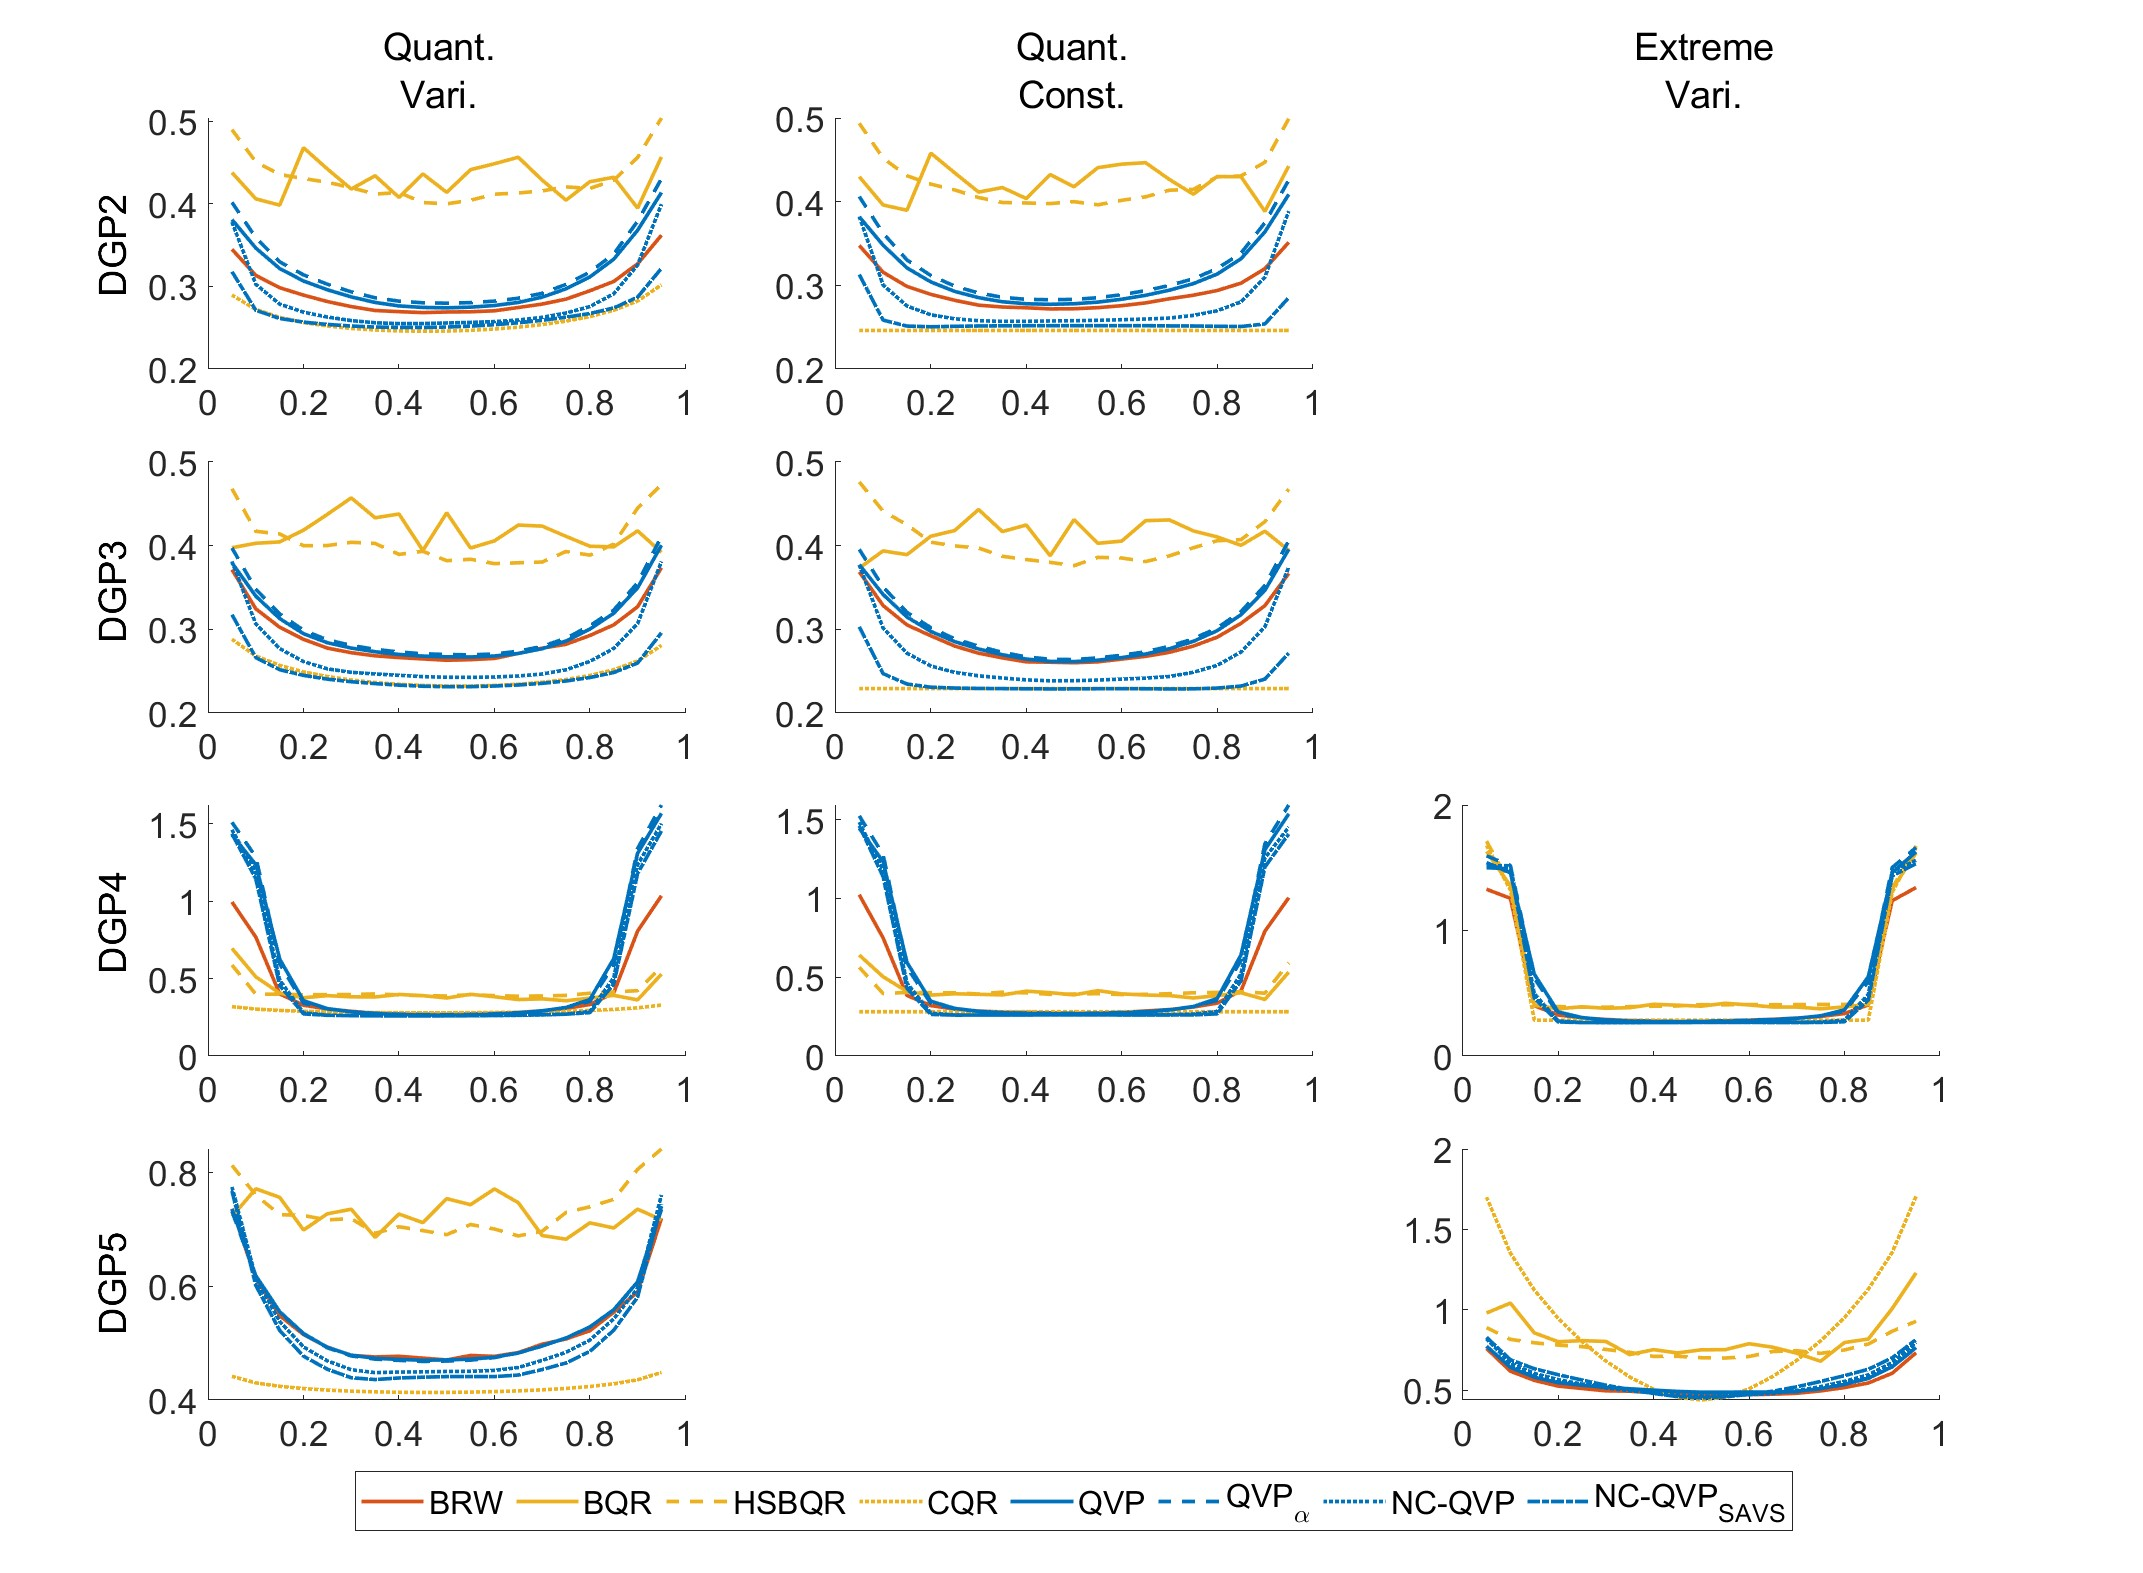
\includegraphics[width=0.9\linewidth]{AppFig/CoeffBiasSpecificv3_alpha.jpg}
    \caption{$\rmse$ profile of $\boldsymbol{\beta}$ across 19 quantiles $\tau_q \in \left\{0.05,\dotsc,0.95\right\}$ for $\mathcal{T}=300$ and $\varDelta$=0. Includes $\QVP_\alpha$. Estimates are based on the posterior mean. }
    \label{fig:AlphaCoeffBias}
\end{figure}

\begin{table}[h!]
\centering
\label{tab:QVP_a}
%\resizebox{\textwidth}{!}{%
\begin{tabular}{lr|c:cc}
 &  & $\BQR$ & $\QVP$ & $\QVP_{\alpha}$ \\ \hline
\multicolumn{2}{l|}{DGP-1} &  &  &  \\
 & $w_1$ & 0.424 & 0.853 & 0.853 \\
 & $w_2$ & 0.078 & 0.906 & 0.906 \\
 & $w_3$ & 0.133 & 0.825 & 0.825 \\
 & $w_4$ & 0.134 & 0.818 & 0.818 \\ \hline
\multicolumn{2}{l|}{DGP-2} &  &  &  \\
 & $w_1$ & 0.432 & 0.843 & 0.845 \\
 & $w_2$ & 0.080 & 0.895 & 0.896 \\
 & $w_3$ & 0.135 & 0.821 & 0.823 \\
 & $w_4$ & 0.138 & 0.804 & 0.806 \\ \hline
\multicolumn{2}{l|}{DGP-3} &  &  &  \\
 & $w_1$ & 0.412 & 0.844 & 0.845 \\
 & $w_2$ & 0.076 & 0.897 & 0.898 \\
 & $w_3$ & 0.132 & 0.799 & 0.800 \\
 & $w_4$ & 0.128 & 0.826 & 0.827 \\ \hline
\multicolumn{2}{l|}{DGP-4} &  &  &  \\
 & $w_1$ & 0.779 & 0.909 & 0.909 \\
 & $w_2$ & 0.141 & 0.941 & 0.941 \\
 & $w_3$ & 0.245 & 0.900 & 0.901 \\
 & $w_4$ & 0.251 & 0.881 & 0.882 \\ \hline
\multicolumn{2}{l|}{DGP-5} &  &  &  \\
 & $w_1$ & 0.716 & 0.880 & 0.880 \\
 & $w_2$ & 0.134 & 0.926 & 0.926 \\
 & $w_3$ & 0.220 & 0.870 & 0.870 \\
 & $w_4$ & 0.228 & 0.837 & 0.837 \\ \hline
\end{tabular}%
%}
\caption{Out-of-sample predictive performance of $\QVP$ vs. $\QVP_{\alpha}$ as measured by the weighted quantile score, $\mathrm{qwQS}$, see Equation~\ref{eq:qwQS}. Performance is shown relative to $\BQR$ whose absolute performance shown above the dotted lines respectively, $\varDelta$=0.0, $\mathcal{T}=300$, $\mathcal{Q}=19$.}
\end{table}

\clearpage

\section{Further Analysis to the Application}\label{app:extra-results-application}


\subsection{Stress Testing}\label{app:stress-testing}
\citet{chavleishvili2024forecasting} outline a method for stress-testing, using a simulation-based procedure for forecasting under stress scenarios using the QVAR framework. Importantly, in the forecasting setup described above and in \citet{chavleishvili2024forecasting} one can also restrict the quantiles to be of a specific sequence for the different variables thereby creating stress-test scenarios. For example, one can impose a series of consecutive tail quantile shocks (e.g., 10\% quantile events) over a designated forecast horizon. This approach leverages the model’s recursive structure to propagate the effect of these extreme shocks forward in time, producing a simulated forecast distribution that reflects potential stress conditions.

This type of analysis is useful because it offers an intuitive depiction of the range of possible outcomes under stress, thereby highlighting the potential magnitude and duration of adverse effects. This is an essential tool in stress testing because they not only illustrate the central forecast under baseline conditions but also reveal the dispersion and asymmetry in the forecast distribution when the system is subjected to extreme shocks. By comparing the stressed forecast paths with baseline forecasts, analysts and policymakers can gain insights into the robustness of the economy and identify periods of heightened vulnerability. This simulation-based approach, rooted in the QVAR framework, thus provides a more comprehensive view of risk by capturing the entire conditional distribution rather than focusing solely on the mean outcome.

Here we note, that on account of the Bayesian framework, we can generate confidence bands around the stress-test scenarios by drawing randomly from the posterior draws. In this way we deviate from \citet{chavleishvili2024forecasting}, and draw randomly from the posterior draws as well to obtain a confidence band around the scenarios. Beyond this difference, everything else is the same as in \citet{chavleishvili2024forecasting}. Namely, the stress scenario is constructed by assuming that the CISS index sees a 0.9 quantile realisation for 6 months followed by median realisations, while the median scenario assumes that both GDP and CISS observe median outcomes across the forecast horizon. The results for IP for the stress-testing scenarios are shown in figure (\ref{fig:StressTest}).\footnote{No bands are constructed for the BRW. This was done because a different procedure would be neccessary to construct these bands than the Bayesian estimators.}

\begin{figure}
    \centering
    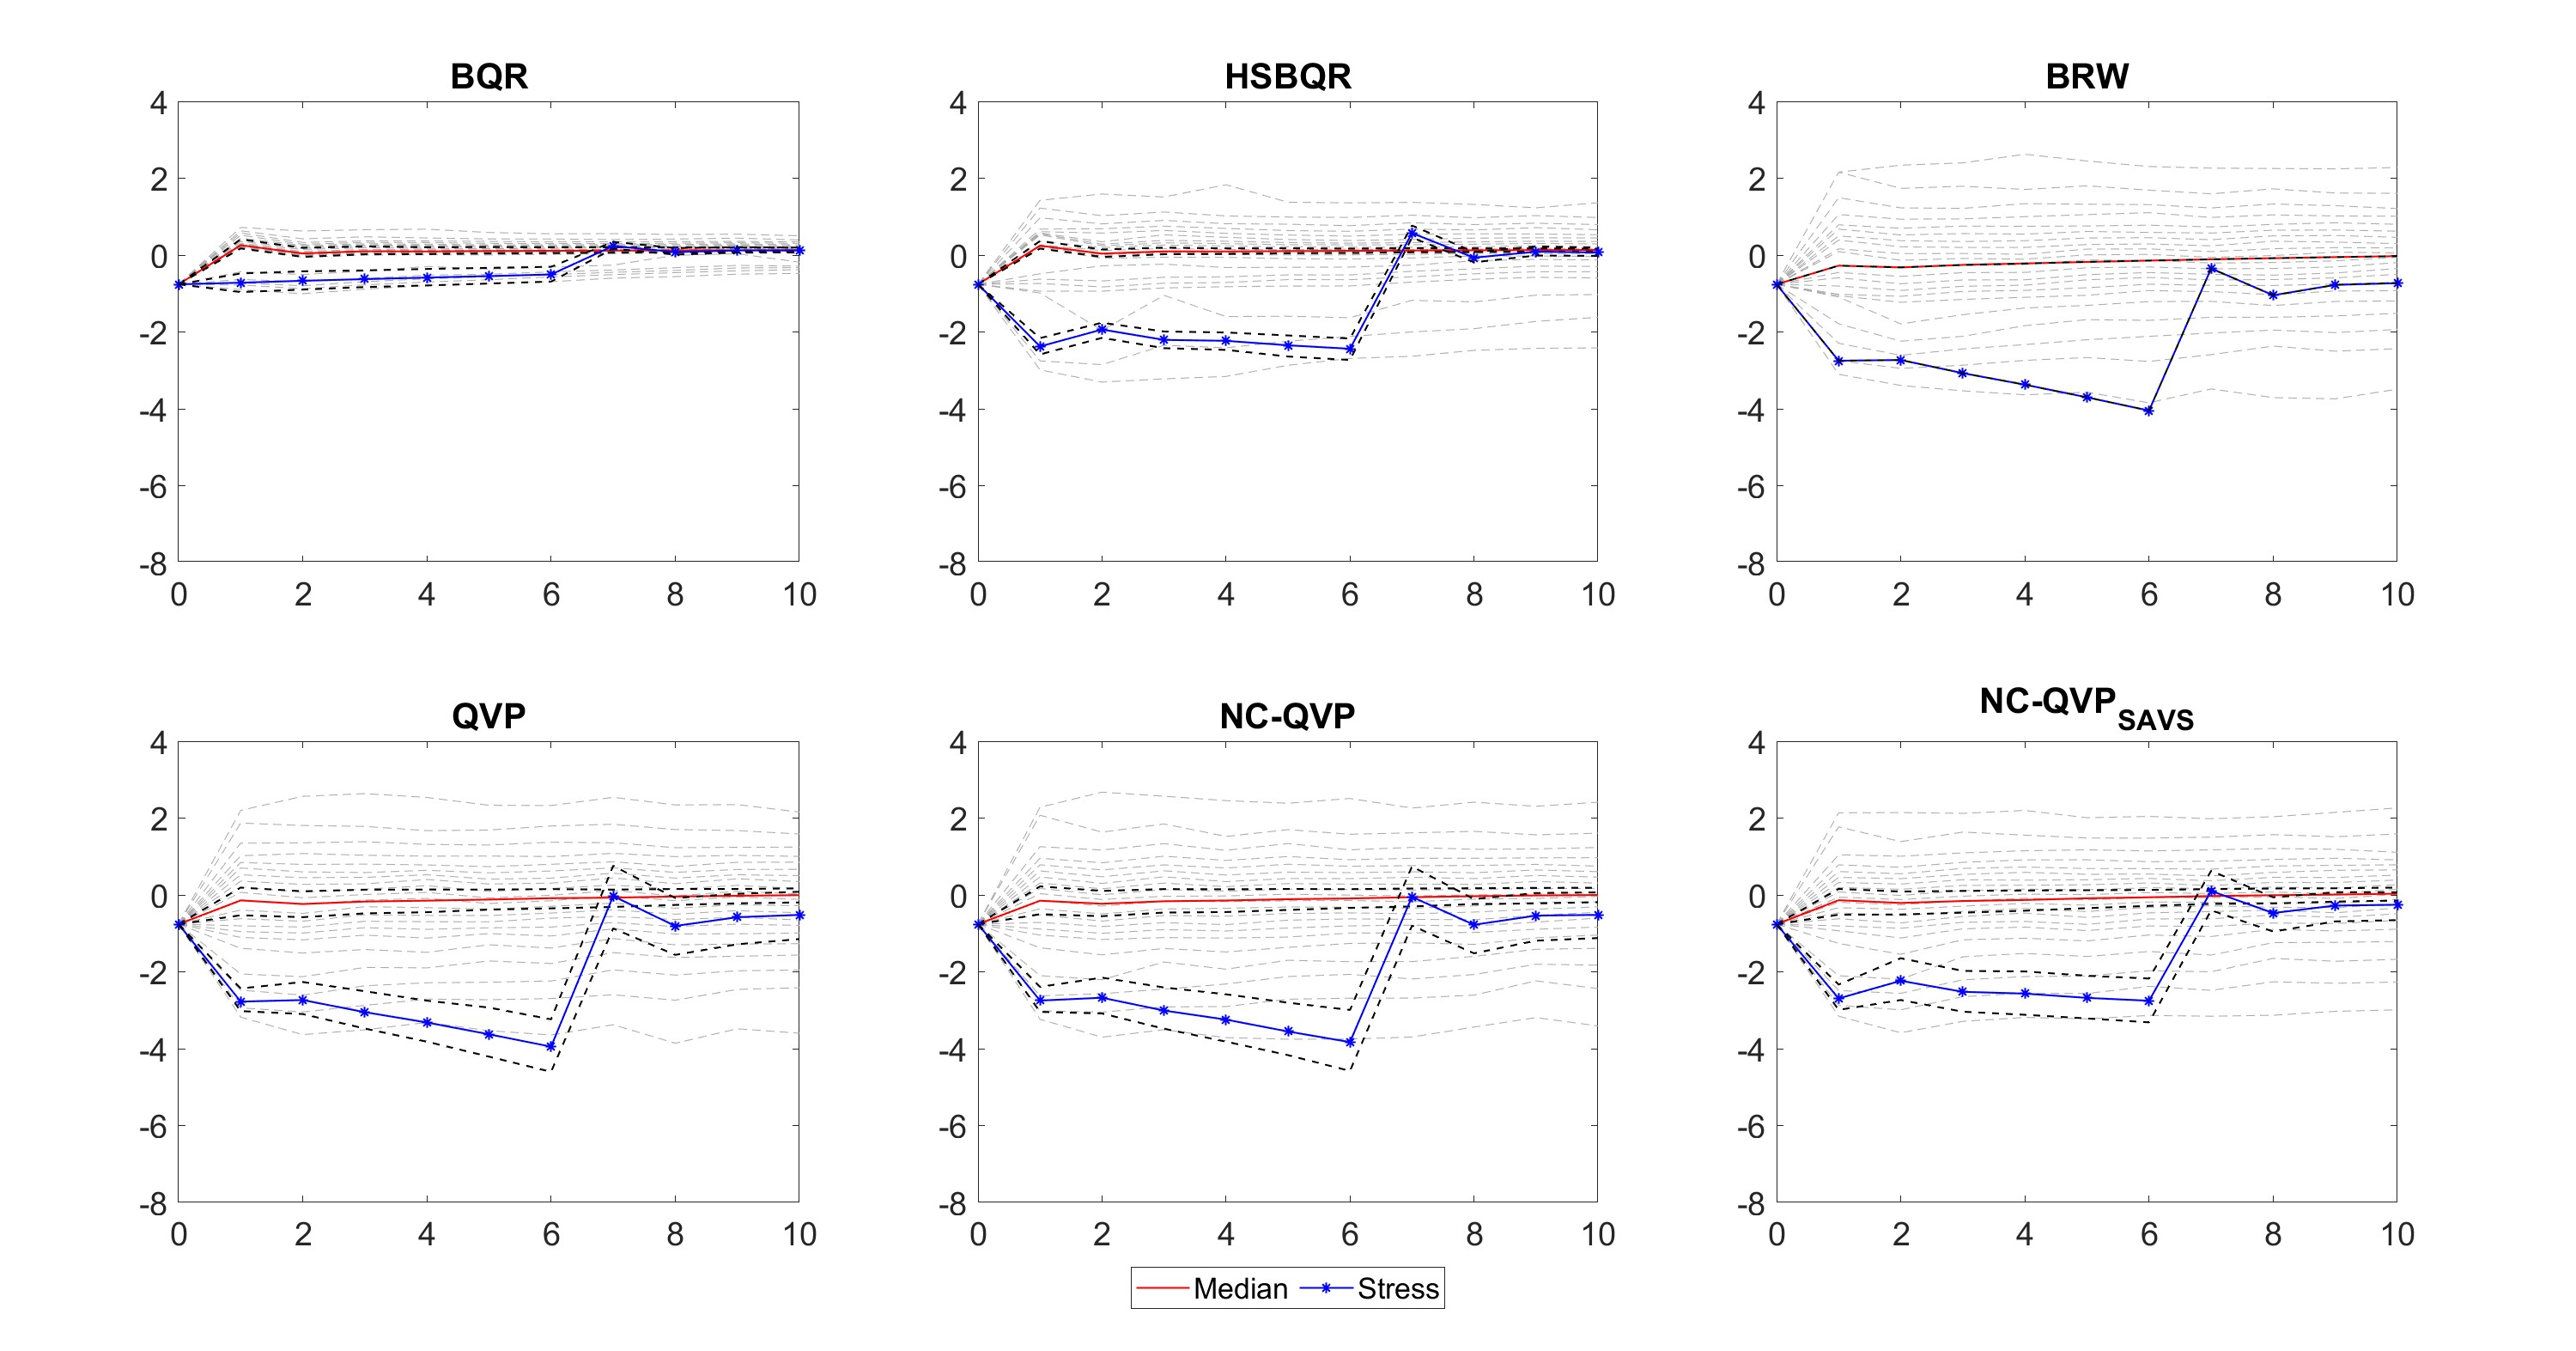
\includegraphics[width=\linewidth]{Figures/Forecast.jpg}
    \caption{Stress-testing}
    \label{fig:StressTest}
\end{figure}

The figure reveals some key differences. First, the BQR produces much lower stress scenarios with narrower spreads, than the other methods. Second, the BRW, QVP, and NCQVP produces very similar profiles, with a sharp drop in IP in $h=1$, followed by a slower decrease in IP growth until $h=6$. Third, the SAVS variant showcase similar profiles as well, but they differ from their non-SAVS counterparts by showing slow recovery from $h=2$ to $h=6$. Finally, while the HSBQR produces a similar stress profile as the joint estimation methods, the stress scenario is not as negative as the joint estimation methods. These highlights how the choice of modelling quantiles jointly (with fused-shrinkage) has a noticeable influence on the outcomes. 

From a policy standpoint, these differences in tail forecasts can significantly influence decisions regarding capital buffers, liquidity requirements, or macroprudential measures. A method that systematically yields tighter stress estimates might understate risks, leading policymakers to adopt insufficient safeguards. Conversely, overly conservative forecasts could prompt more stringent policies, potentially dampening economic activity. By comparing a range of models and stress outcomes, policymakers can better triangulate the severity of risks, ensuring that policy interventions strike a balance between prudence and efficiency.

\subsection{Coefficient Posteriors}\label{app-sec:fig-posteriors}{\color{white}.}

\begin{figure}[H]
     \centering
     \begin{subfigure}[b]{\textwidth}
         \centering
         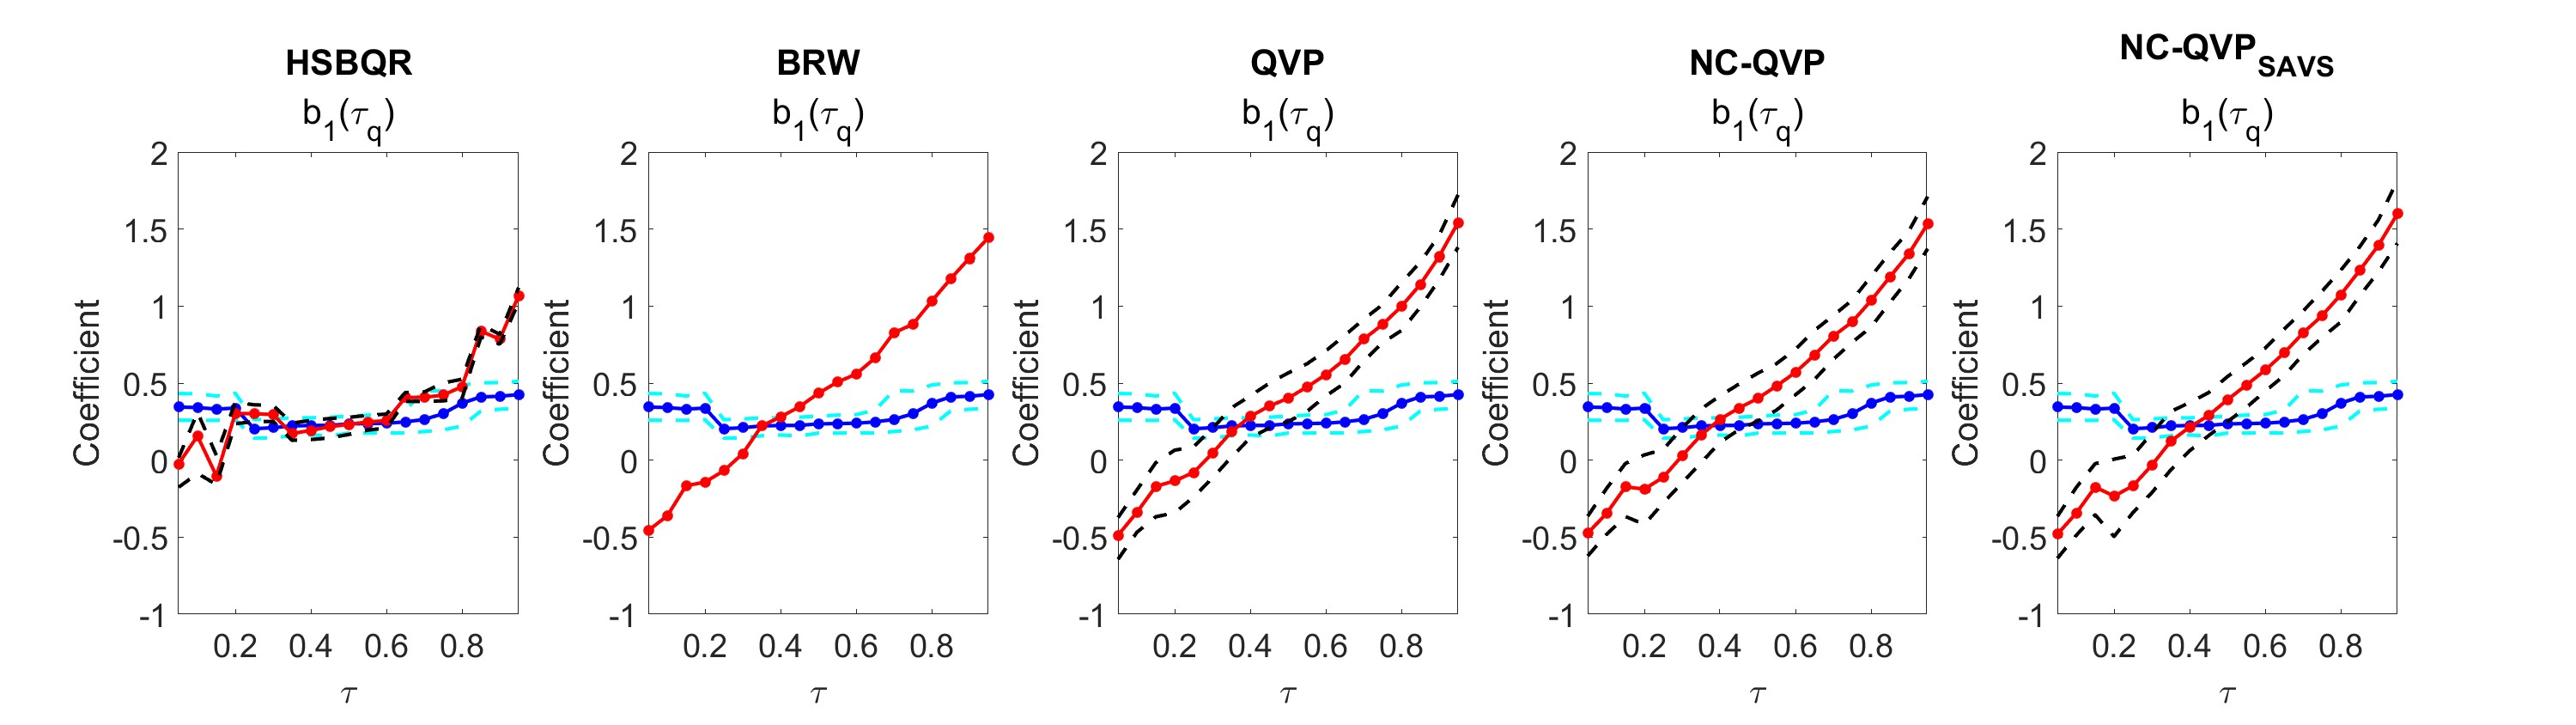
\includegraphics[width=\textwidth]{Figures/FigureCoeff1.jpg}
     \end{subfigure}
     \vfill
     \begin{subfigure}[b]{\textwidth}
         \centering
         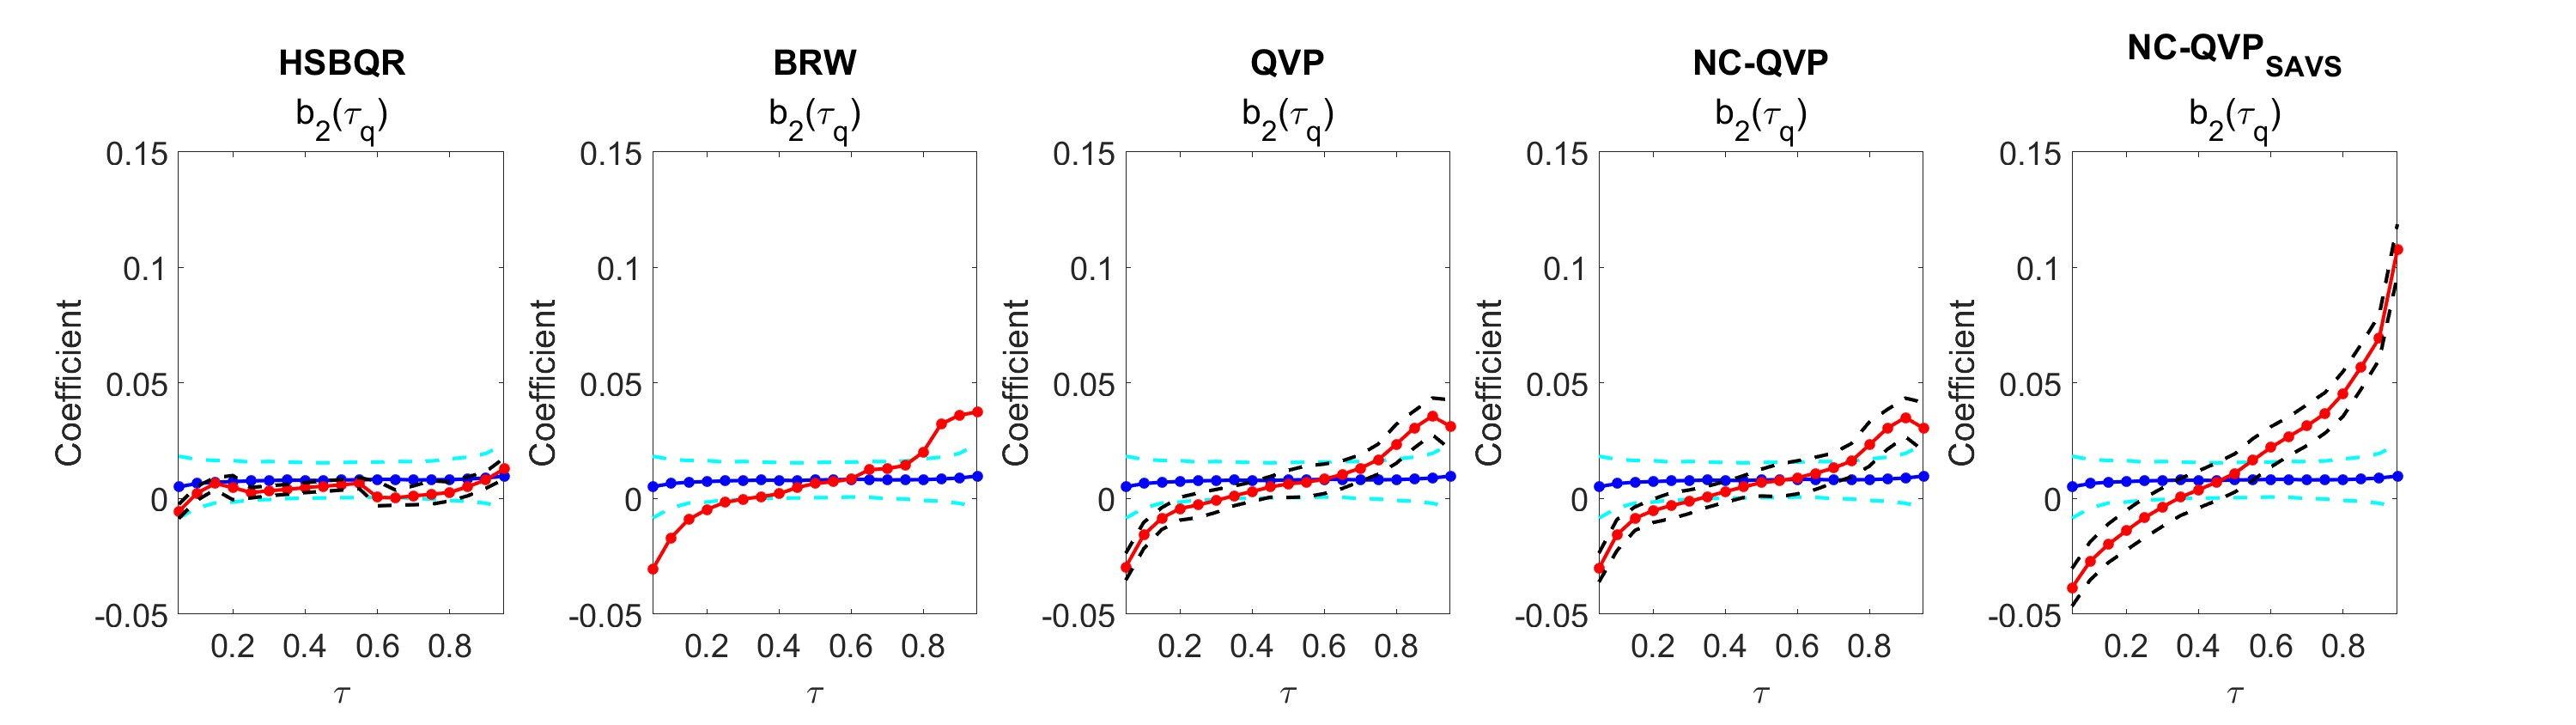
\includegraphics[width=\textwidth]{Figures/FigureCoeff4.jpg}
     \end{subfigure}
        \caption{Intercept posteriors}
        \label{fig:CoeffsIntercept}
\end{figure}

\begin{figure}[H]
    \centering
    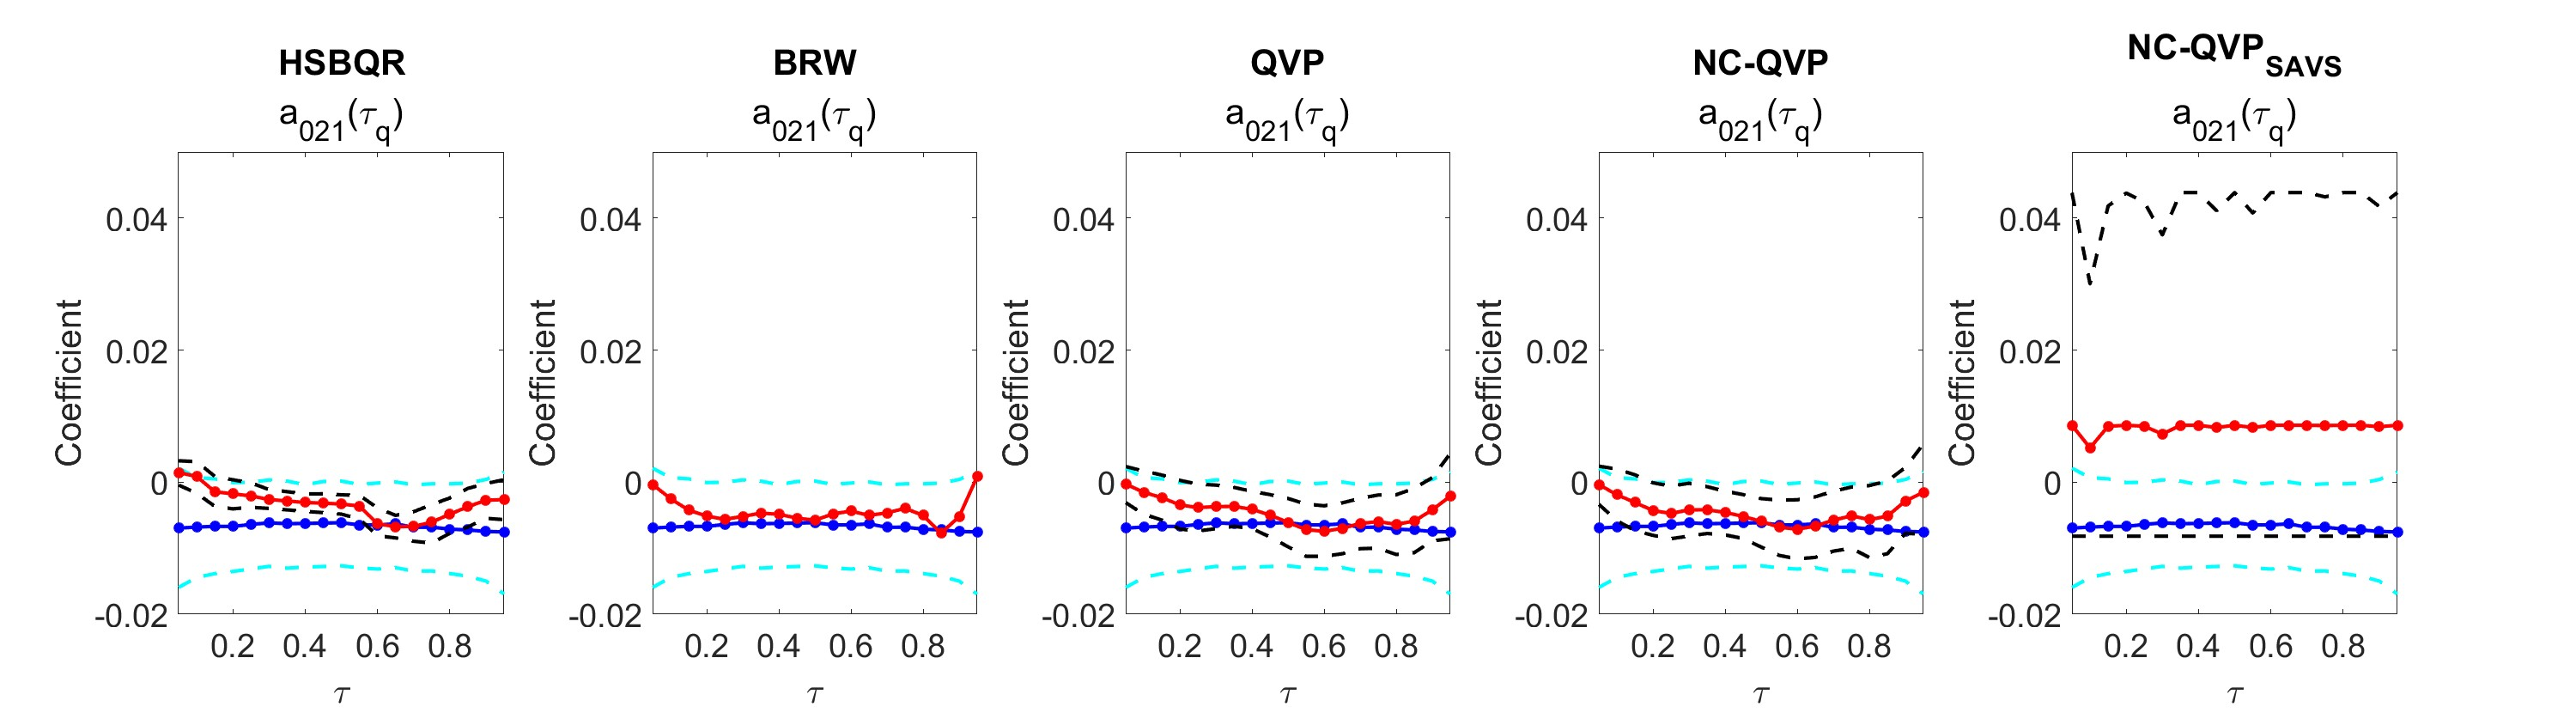
\includegraphics[width=\linewidth]{Figures/FigureCoeff7.jpg}
    \caption{Contemporaneous effect posteriors}
    \label{fig:CoeffsContemp}
\end{figure}

\begin{figure}[H]
     \centering
     \begin{subfigure}[b]{\textwidth}
         \centering
         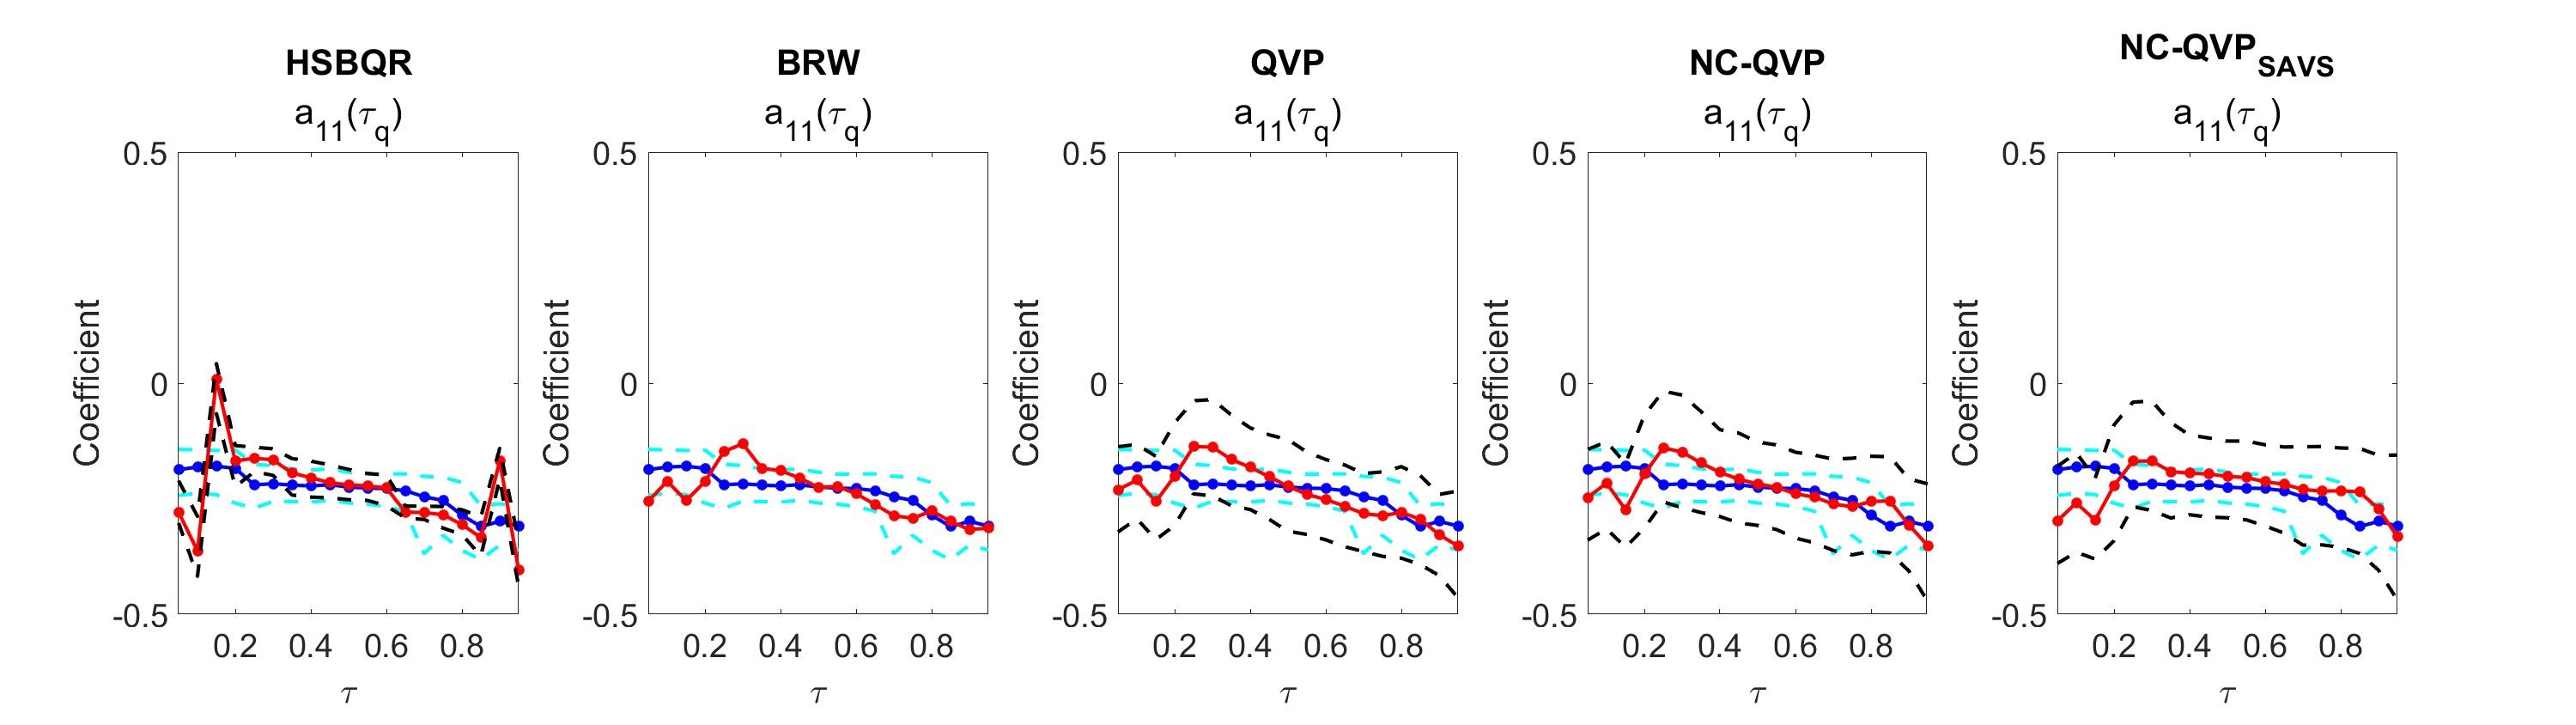
\includegraphics[width=\textwidth]{Figures/FigureCoeff2.jpg}
     \end{subfigure}
     \vfill
     \begin{subfigure}[b]{\textwidth}
         \centering
         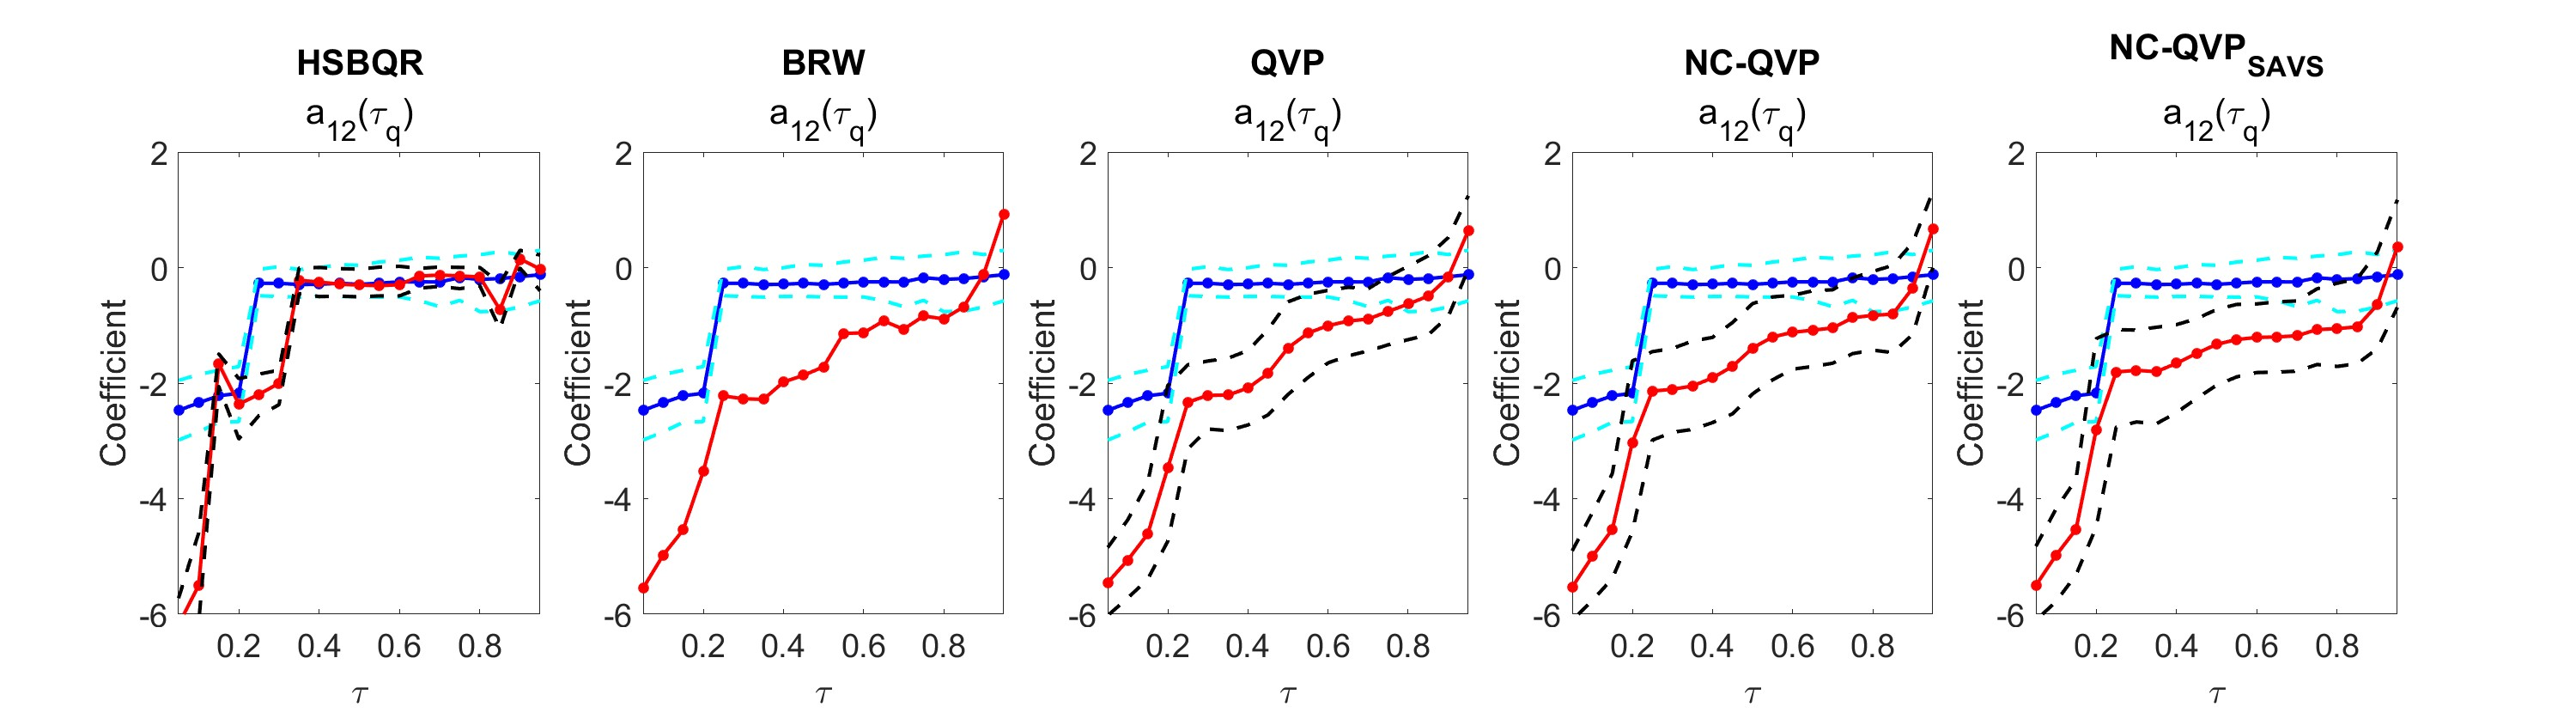
\includegraphics[width=\textwidth]{Figures/FigureCoeff3.jpg}
     \end{subfigure}
     \vfill
     \begin{subfigure}[b]{\textwidth}
         \centering
         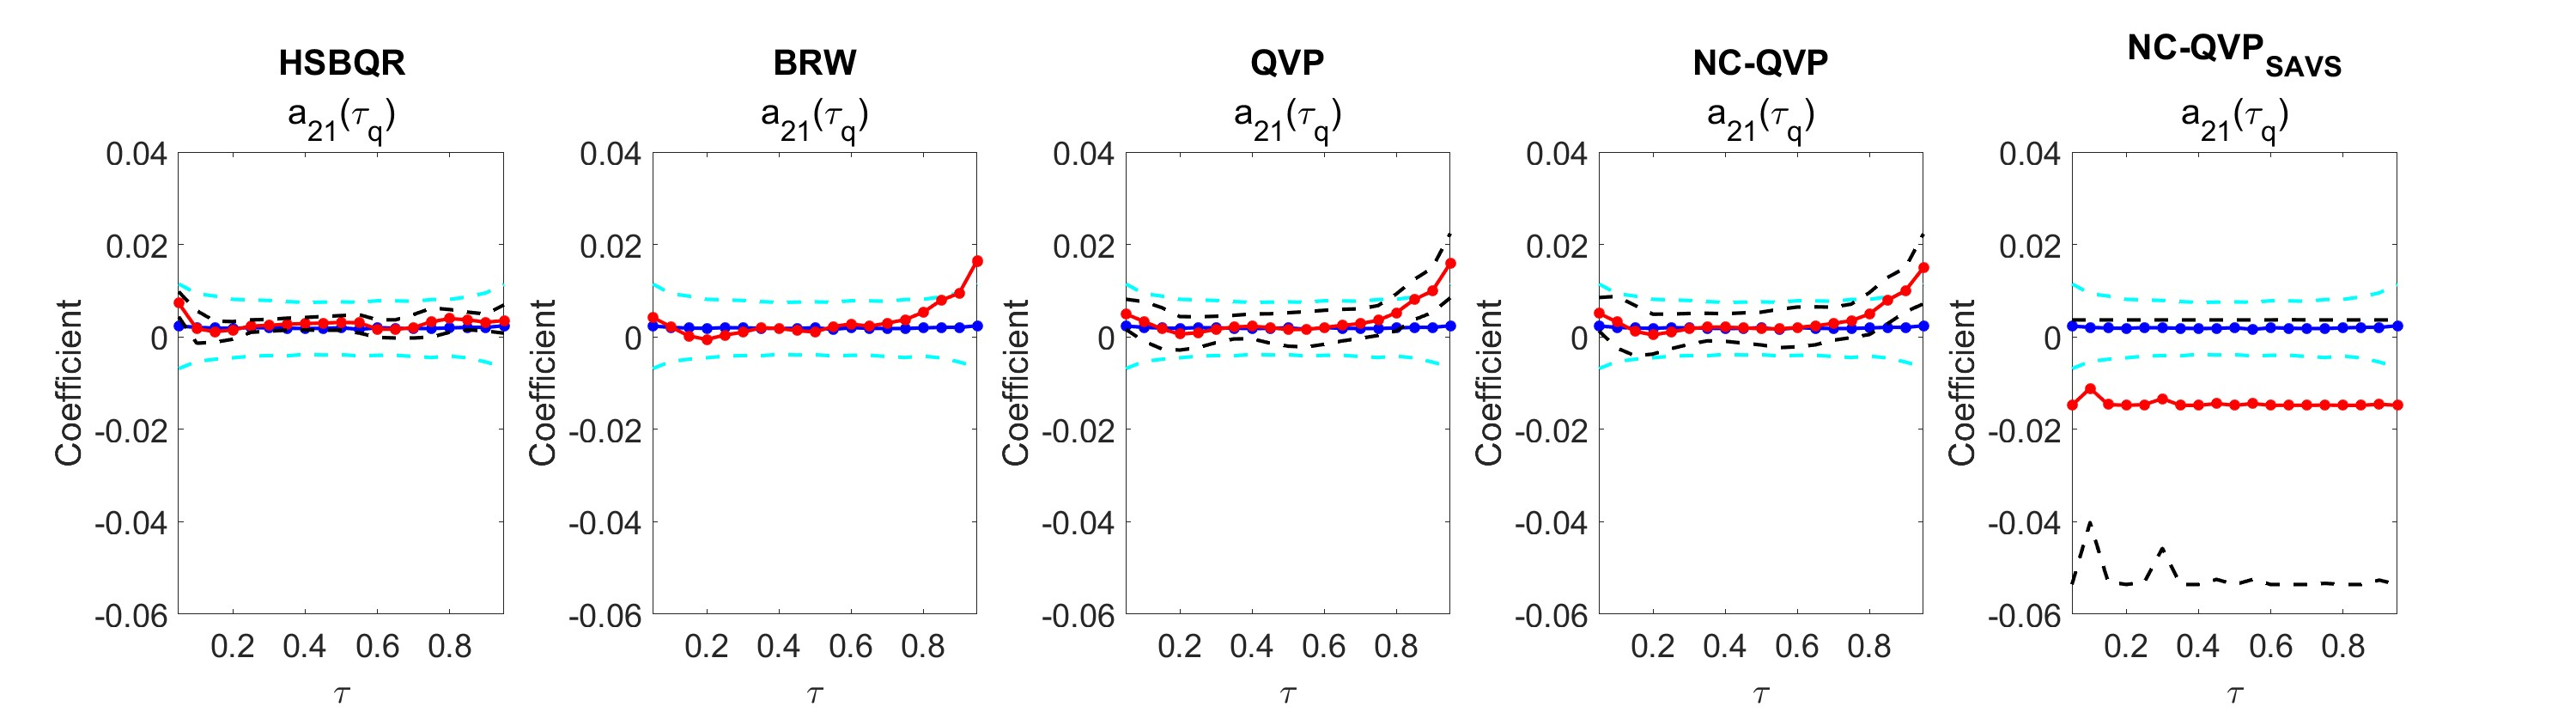
\includegraphics[width=\textwidth]{Figures/FigureCoeff5.jpg}
     \end{subfigure}
     \vfill
     \begin{subfigure}[b]{\textwidth}
         \centering
         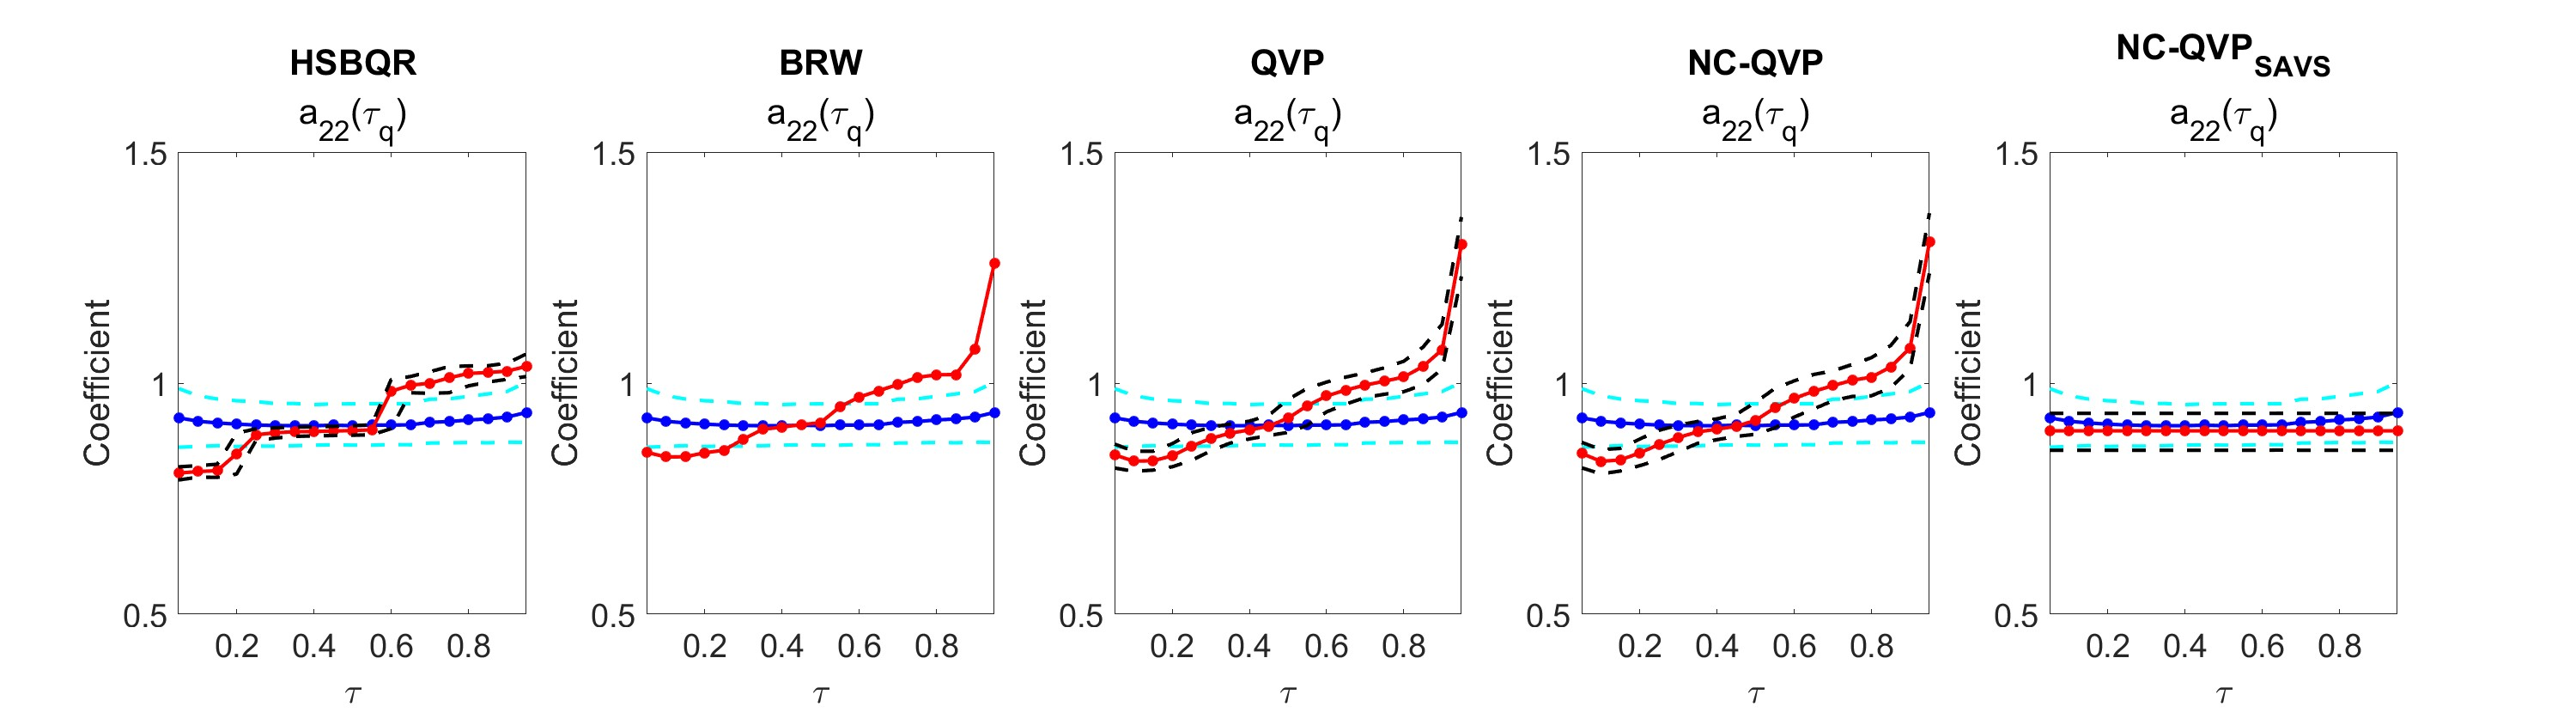
\includegraphics[width=\textwidth]{Figures/FigureCoeff6.jpg}
     \end{subfigure}
        \caption{Lagged effects posteriors}
        \label{fig:CoeffsLag}
\end{figure}